% ================================================================
% CHAPTER 4: Lösung
% ================================================================

	
\chapter{Lösung}

\section{Codierung von Domänenwissen}

Tabelle xx (<<VERWEIS AUF TABELLE EINFÜGEN>>) codiert Domänenwissen von Tierärzten, welches für die Geburtsprognose von Bedeutung ist. Expertenwissen ist so codiert, dass jedes Geburtsmerkmal mit einer Gewichtung versehen ist. Somit hat das Merkmal an Stelle $i$ die Gewichtung $\lambda_{i}$.



Wie in Formel \ref{Linerarkombination zur Geburtsprognose} formalisiert, werden bei Erkennung eines oder mehrerer Merkmale in einem Bild, die Gewichtungen dieser Merkmale addiert. Merkmale, welche als Geburtsanzeichen dienen, haben eine positive Gewichtung und erhöhen dadurch das Endergebnis. Merkmale, welche darauf hinweisen, dass zurzeit keine Entbindung stattfindet, haben eine negative Gewichtung und senken das Endergebnis.


Das Resultat dieser Berechnung bezeichnet der Autor als \flqq qualitative Situationsbewertung\frqq. Diese wird mit einem Schwellwert verglichen, um zu entscheiden, ob eine Benachrichtigung verschickt wird.

Dabei kann die qualitative Situationsbewertung anhand der folgenden Linearkombination ermittelt werden: 



\begin{equation}\label{Linerarkombination zur Geburtsprognose}
v = h(x) = \sum_{i=1}^n \lambda_{i}*x_{i}
\end{equation}

 
Wobei $\lambda_{i}$ sich aus der fachlichen Gewichtung $\kappa_{i}$ und der technischen Qualitätsbeurteilung $\beta_{i}$ zusammensetzt. Die Skala zur Bewertung reicht von -10 bis 10, daher ergibt sich $ \lambda = \kappa = \beta = \{ \:  m \: | \:  m \:  \varepsilon \:  \mathbb{Z}, -10 \:  \leq \: m \: \leq \:  10\} $.

Die fachliche Gewichtung eines Merkmals entspricht der Bewertung  der Stärke des Hinweises in Bezug auf eine bevorstehende Geburt. Dementsprechend codiert $\kappa$ Domänenwissen von Tierärzten zur merkmalsbezogene Einschätzung und Prognose des Geburtsverlaufs.

Die technische Qualitätsbeurteilung basiert auf der Güte der technischen Mittel zwecks Analyse der An- oder Abwesenheit eines Merkmals in einem Bild. Dementsprechend wird $\beta$ benötigt, weil nicht sämtliche Merkmale mit derselben Qualität auf deren An- oder Abwesenheit überprüft werden können.

Zwischen den beiden Gewichtungen $\kappa$ und $\beta$ existiert eine schwache Beziehung. Dies wird dadurch begründet, dass technische Zuverlässigkeit die Anwesenheit eines Merkmals nicht überbewerten soll. Beispielsweise soll eine besonders hohe technische Qualitätsbeurteilung und eine tiefe fachliche Gewichtung nicht in einer hohen Gewichtung resultieren. Um diese zwei Gewichtungen schwach miteinander in Beziehung zu setzen, werden diese addiert und nicht multipliziert. Es gilt also: $\lambda_{i} = \kappa_{i} + \beta_{i}$

Zudem codiert $x_{i}$ die Anwesenheit ($x_{i}=1$) oder die Abwesenheit ($x_{i}=0$) eines spezifischen Merkmals auf einem Bild. Es gilt dementsprechend  $ x_{i} \:  \varepsilon \: \{0,1\}. $ 


Setzen wir diese Erkenntnisse zusammen, so ergibt sich

\begin{equation}\label{Vollständige Linerarkombination zur Geburtsprognose}
v = h(x) = \sum_{i=1}^n (\kappa_{i}+\beta_{i}) *x_{i}
\end{equation}

wobei:  $ x \:  \varepsilon \: \{0,1\} $ und $\kappa = \beta = \{ \:  m \: | \:  m \:  \varepsilon \:  \mathbb{Z}, -10 \:  \leq \: m \: \leq \:  10\} $.

Das Ergebnis dieser Rechenoperation ergibt wie bereits erwähnt die qualitative Situationsbewertung $v$, welche mit einem Schwellwert verglichen wird. Dies wird formal wie folgt ausgedrückt:

\begin{equation}\label{Vollständige Linerarkombination zur Geburtsprognose: Schwellwertanalyse}
y = g(v) =\begin{cases}
			1,\: wenn \: v > q\\
			0,\: wenn \: v \leq q
\end{cases}
\end{equation}

Dabei steht $q$ für den Schwellwert, welcher in der Domänenanalyse ermittelt wird. Das Ergebnis $y=1$ bedeutet, dass eine Benachrichtigung ausgelöst wird, während bei $y=0$ keine Benachrichtigung ausgelöst wird.

 






\newgeometry{margin=2.5cm} % Ränder kleiner	
\begin{landscape}

\section{Modellierung der Lösung}
Für die Dokumentation der Lösung verwendet der Autor die UML-Notation. Zwei Kassendiagramme beschreiben das System aus jeweils unterschiedlichen Perspektiven \cite{Uml-modellierung2012}. 

\subsection{Klassendiagramm des Pakets Image-Analysis }
\begin{figure}[H]
	\center
	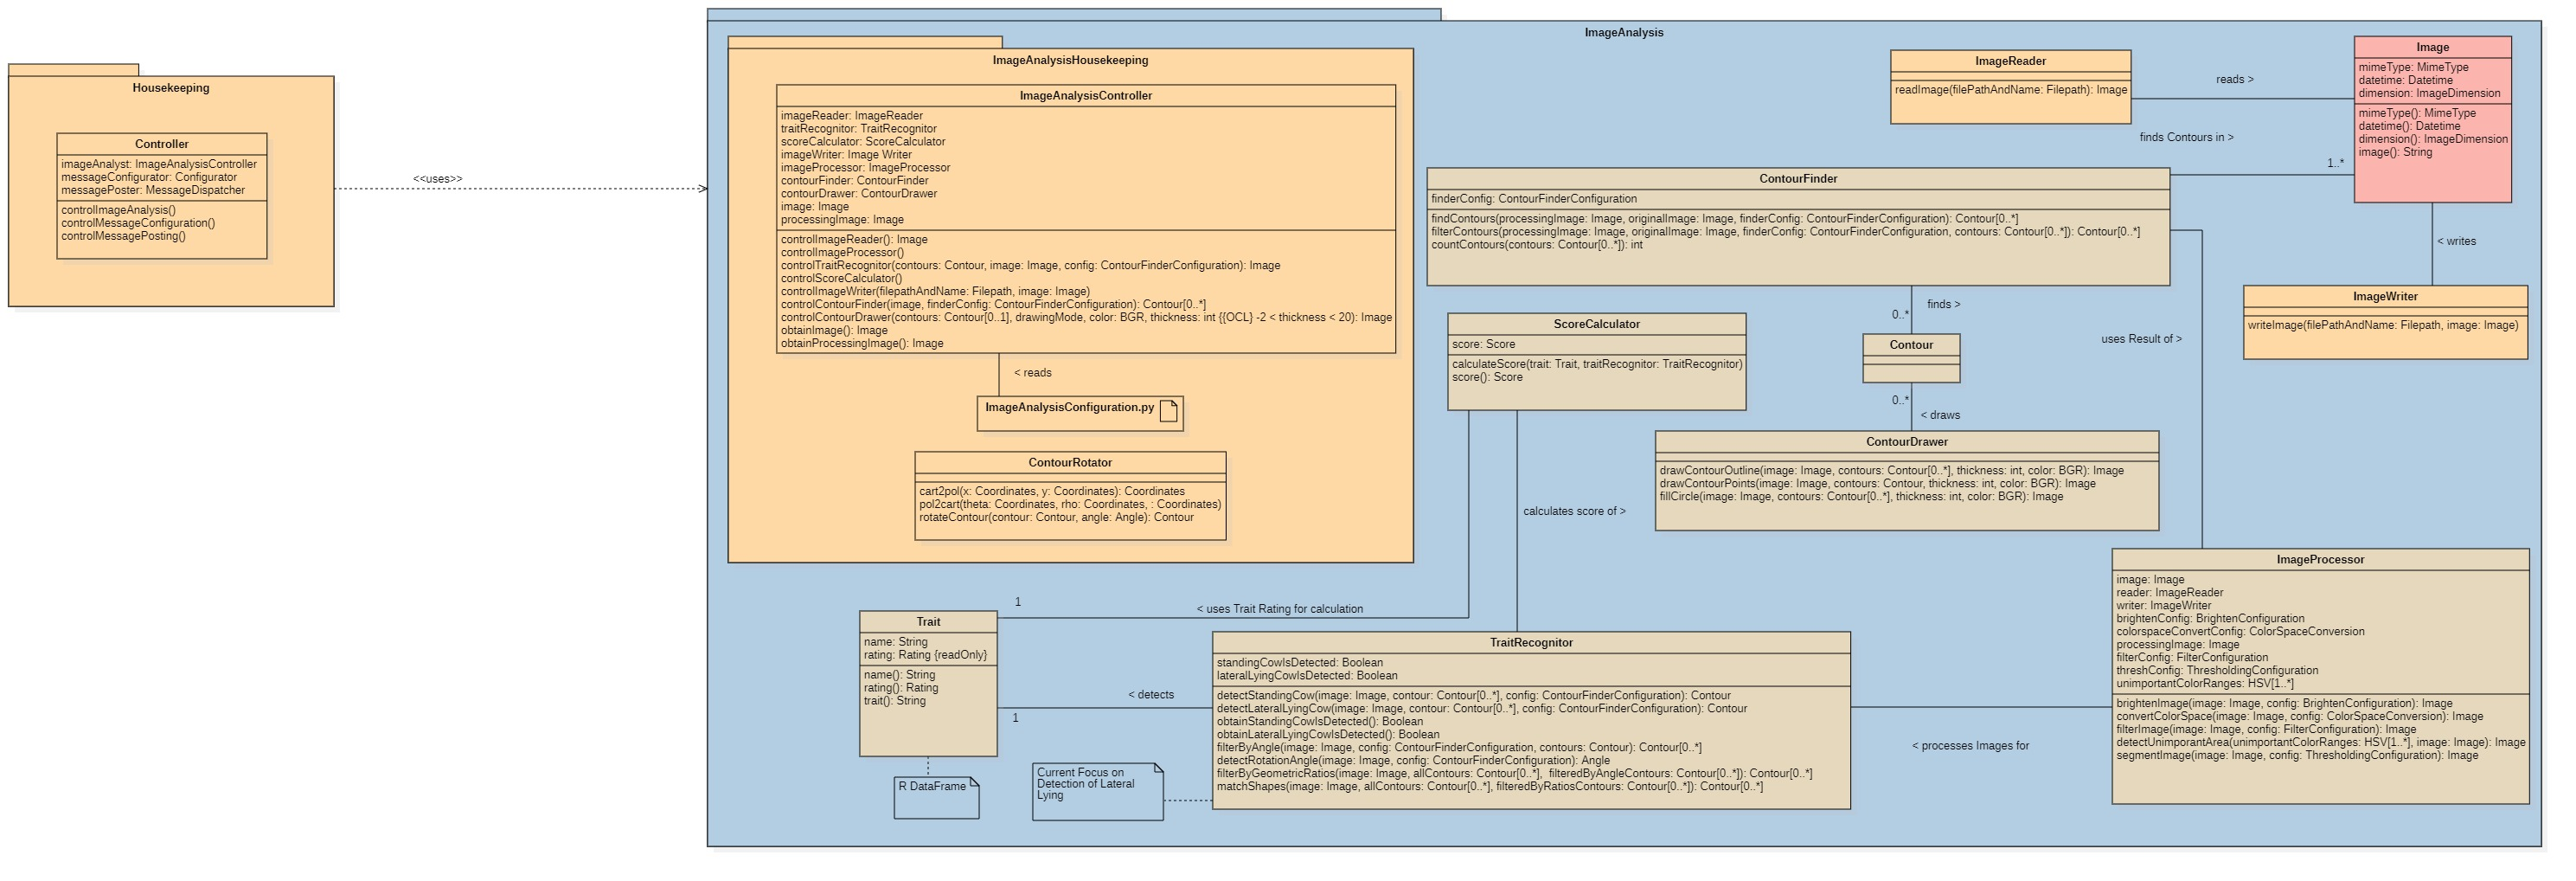
\includegraphics[scale=0.45]{Grafiken/modelle/solution-imageanalysis.jpg}
	\caption{Lösungsdokumentation des Pakets Image-Analysis zur Geburtsprognose und Geburtserkennung.} 
	\label{fig: Lösungsdokumentation des Pakets Image-Analysis zur Geburtsprognose und Geburtserkennung.}
\end{figure}

\subsection{Klassendiagramm der Pakete Message-Configuration und Message-Posting}
\begin{figure}[H]
	\center
	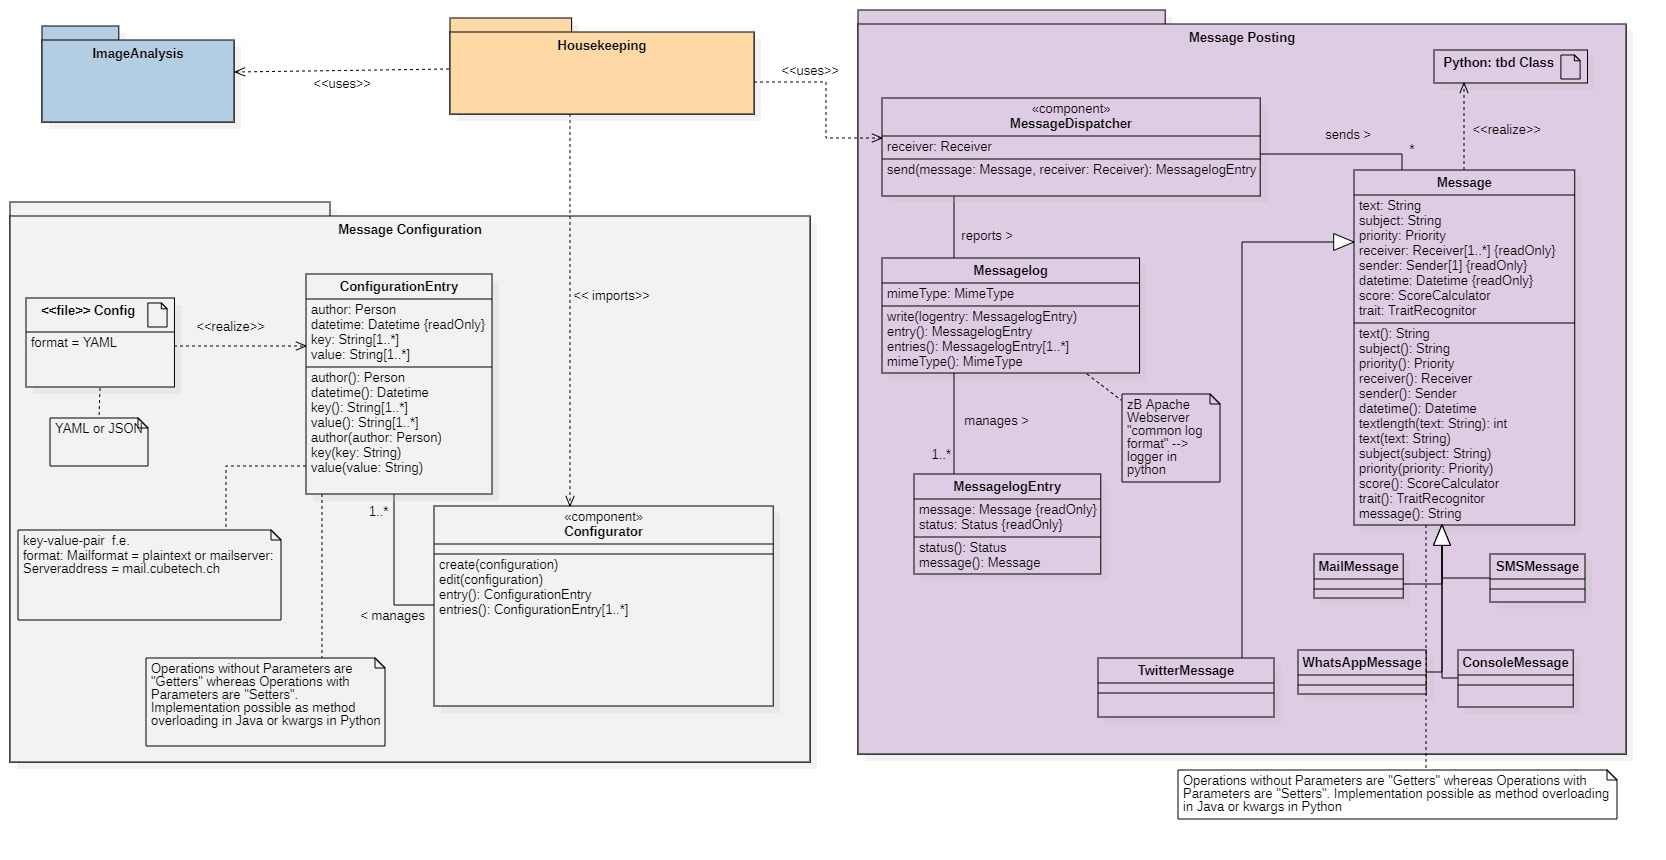
\includegraphics[scale=0.43]{Grafiken/modelle/solution-messaging.jpg}
	\caption{Lösungsdokumentation der Pakete Message-Configuration zur Konfiguration und Message Posting zum Versand von Benachrichtigungen.} 
	\label{fig: Lösungsdokumentation der Pakete Message-Configuration zur Konfiguration und Message Posting zum Versand von Benachrichtigungen.}
\end{figure}

\subsection{Value-Object-Bibliothek}
Die Bibliothek an Value Objects wird gemäss Kapitel 3 Domänenanalyse eingesetzt.

Zusammenfassend ist erwähnenswert,... 

\end{landscape}
\restoregeometry % Wieder die alten Ränder

\section{Überlegungen für den Betrieb}

Um einen stabilen Betrieb von elektronischen Geräten und dem Netzwerk auf einem Bauernhof sicherzustellen, müssen folgende Überlegungen gemacht werden:


\newpage


\section{Umsetzung in Entwicklung}
Um die schrittweise Entwicklung und entsprechende Teilergebnisse der Bildbearbeitung zu veranschaulichen, dient Abbildung \ref{fig: Ausgangslage für die Bildanalyse} als Ausgangsbild. Dieses Bild wurde vom System erstellt, welches im Rahmen der erwähnten Case-Arbeit entwickelt wurde. Anschliessend wurde das Bild mit der Funktion \texttt{add()} heller gemacht und unter Anwendung von \texttt{createCLAHE()} und \texttt{clahe.apply()} wurde das Histogramm des Bildes geglättet. 

\begin{figure}[H]
	\center
	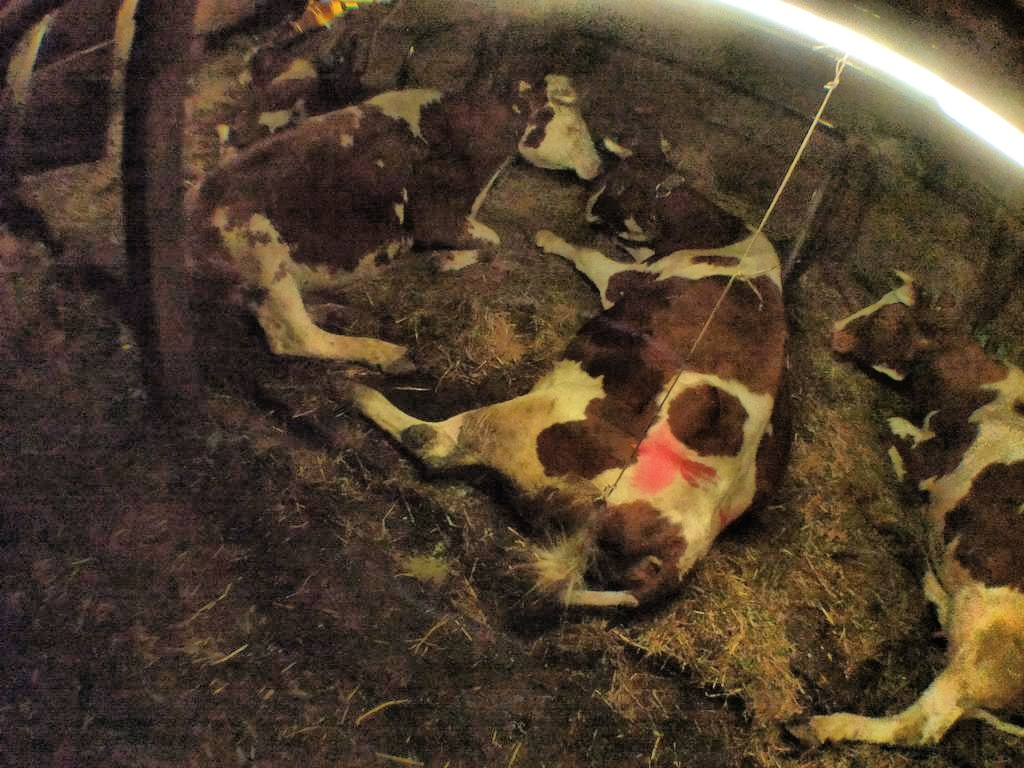
\includegraphics[scale=0.43]{Grafiken/entwicklung/1ausgangsbildBericht.jpg}
	\caption{Beispielbild als Ausgangslage zur Veranschaulichung des Vorgehens} 
	\label{fig: Ausgangslage für die Bildanalyse}
\end{figure}

Abbildung \ref{fig: Vergleich der Histogramme vor und nach Bildbearbeitung} zeigt auf der linken Seite das Histogramm des Originalbilds und auf der rechten Seite das Histrogramm des aufgehellten und geglätteten Bilds. Dabei fällt auf, dass aufgrund der Aufhellung des gesamten Bildes im Histogramm der Wertebereich nach rechts verschoben wird. Zudem sind als Folge der Glättung des Histogramms mittels CLAHE\footnote{Contrast Limited Adaptive Histogram Equalization} die Anzahl Pixel weniger stark auf einen Bereich konzentriert. CLAHE ist ein Verfahren, dass für die Glättung von Bildern und Verbesserung des Kontrasts eingesetzt wird. Ein Vorteil der Methode ist, dass aufgrund einer parametrisierbaren Begrenzung der Kontrastverstärkung die Überbetonung von Rausch in relativ homogenen Regionen des Bilds verhindert wird \citep[S. 313]{FernandezVillan2019}.

Das Bild \ref{fig: Ausgangslage für die Bildanalyse} wird nun unter Anwendung von diversen Methoden aus der Bildanalyse und der Software-Bibliothek OpenCV bearbeitet und analysiert, um daraus Information zum Geburtsverlauf eines Kalbes zu gewinnen. In der vorliegenden Arbeit liegt der Fokus in der Detektierung von seitlichem Liegen, da die Erkennung dieses Geburtsmerkmals einen hohen Mehrwert bringt. 

\begin{figure}[H]
	\center
	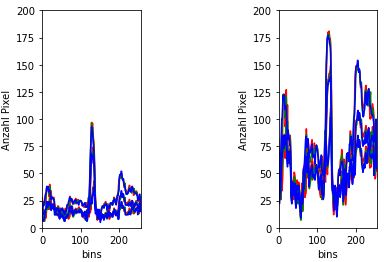
\includegraphics[scale=0.9]{Grafiken/entwicklung/2HistrogrammVergleich.jpg}
	\caption{Vergleich der Histogramme vor und nach Bildbearbeitung} 
	\label{fig: Vergleich der Histogramme vor und nach Bildbearbeitung}
\end{figure}

\subsection{Detektierung von unwichtigen Bereichen im Bild}
Um das Potential aus der Detektierung von unwichtigen Bereichen zu veranschaulichen, wird in einem ersten Schritt ein Binärbild des Originalbilds erstellt. Dazu wird die Funktion \texttt{threshold()} mit dem Verfahrentyp \texttt{THRESH_BINARY} und dem Wert \texttt{40} als Schwellwert eingesetzt. OpenCV ermöglicht mit der Funktion \texttt{threshold()}, die Segmentierung des Bild. Das Bild wird in eine Repräsentation umgewandelt, welche sich für die Weiterverarbeitung besser eignet als die ursprüngliche. \cite[S.328-335]{FernandezVillan2019} In der vorliegenden Arbeit basiert die Extraktion von Objekten darauf, dass durch Schwellwertverfahren bestimmte Eigenschaften wie Farben und Ecken extrahiert werden können. Die Auswahl vom Wert \texttt{40} als Schwellwert hat zur Folge, dass Pixel mit einer Intensität kleiner gleich \texttt{40} im resultierenden Bild schwarz dargestellt werden und alle anderen Pixel weiss. Als Bild zur Eingabe dient ein Graustufenbild. Grundsätzlich können mithilfe des Parameter \texttt{maxval} bei Erreichung des Schwellwerts auch Graustufen als Zielwert für einen Pixel zugewiesen werden. Da in der vorliegenden Arbeit das Schwellwertverfahren aber zur zur Vorbereitung für \texttt{findContours()} gemacht wurde, bringt dies keinen Mehrwert. Da die Funktion \texttt{findContours()} sämtliche Pixel, die nicht den Wert \texttt{0} haben, den Wert \texttt{1} zuweist, wird auch ein Bild mit Graustufen als Binärbild behandelt \cite[S. 366]{FernandezVillan2019}. 

\begin{equation}\label{Vollständige Linerarkombination zur Geburtsprognose: Schwellwertanalyse}
dst(x,y) =\begin{cases}
maxval,\: if \: src(x,y) > thresh\\
0\: otherwise
\end{cases}
\end{equation}

Nebst der Funktion \texttt{threshold()} und dem Typ \texttt{THRESH_BINARY} bietet OpenCV weiteren Typen wie \texttt{THRESH_BINARY_INV} oder \texttt{THRESH_TRUNC} und das adaptive Schwellwertverfahren \texttt{adaptiveThreshold()} an. Adaptive Schwellwertverfahren ermöglichen den Einsatz von spezifischen Schwellwerten auf Basis einer Gruppe von benachbarten Pixeln  \cite[S.342 f]{FernandezVillan2019}. Die im Rahmen der Bachlor-Arbeit entwickelte Lösung unterstützt die Parametrisierung dieser Funktionen mittels Enumerations. Diese haben aber für die vorliegende Bildanalyse jedoch keine zentrale Bedeutung und werden deshalb nicht weiter erläutert.

\begin{figure}[H]
	\center
	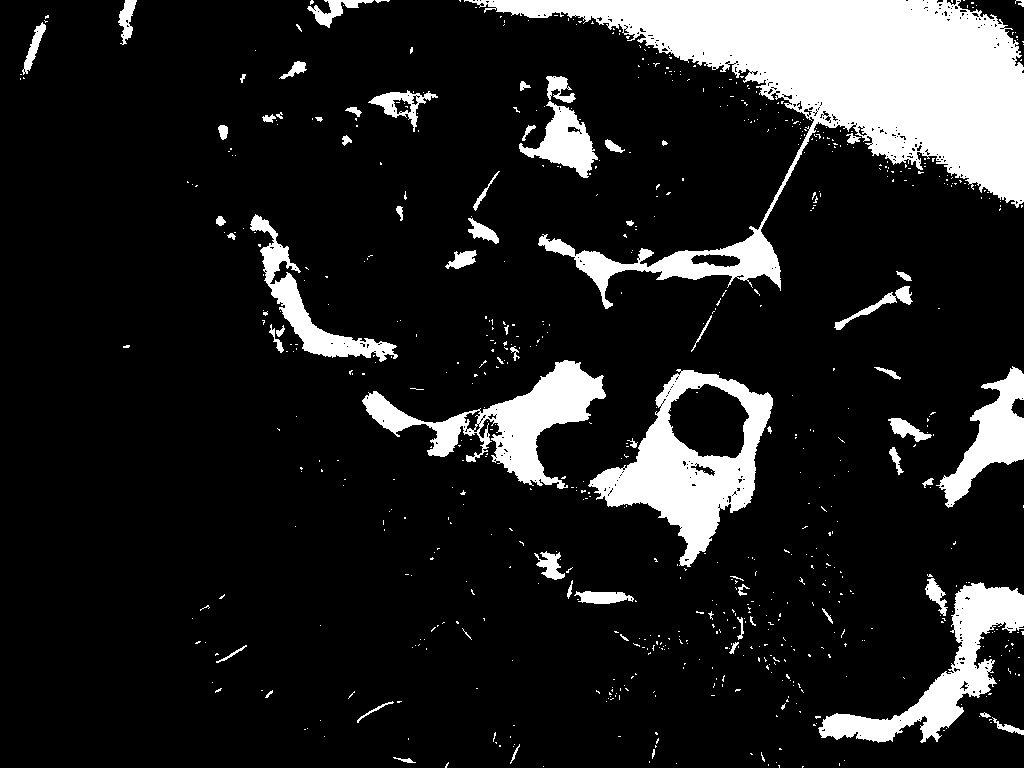
\includegraphics[scale=0.43]{Grafiken/entwicklung/8thresholdedMask.jpg}
	\caption{Binärbild vom Originalbild als Resultat vom Schwellwertverfahren} 
		\label{fig: Binärbild vom Originalbild als Resultat vom Schwellwertverfahren}
\end{figure}
		
In diesem Binärbild werden anschliessend mit den Funktionen \texttt{findContours()} und \texttt{drawContours()} Konturen gesucht und im Originalbild eingezeichnet. Die Funktion \texttt{findContours()} wird verwendet, um Konturen in einem Binärbild zu erkennen. Der Algorithmus unterstützt unterschiedliche Modi wie \texttt{RETR_EXTERNAL} für die Beschränkung auf äussere Konturen, \texttt{RETR_LIST} für die Ausgabe sämtlicher Konturen ohne Hierarchie oder \texttt{RETR_TREE} für die zusätzliche Ausgabe von Informationen zur Hierarchie der Konturen. 

\begin{figure}[H]
	\center
	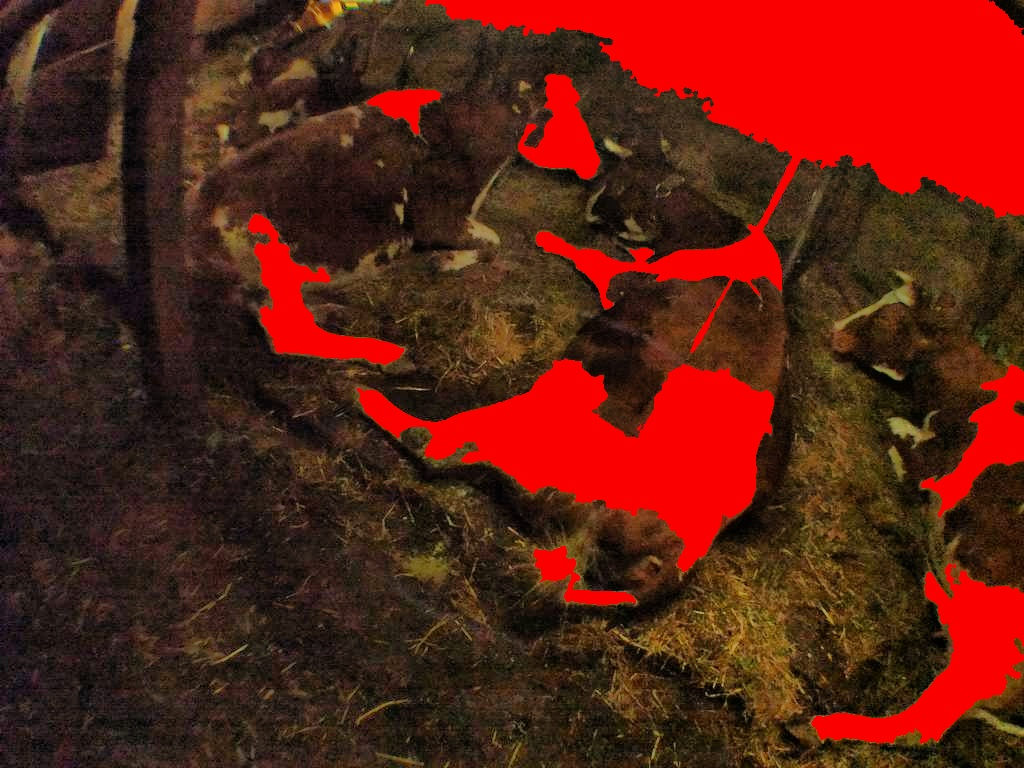
\includegraphics[scale=0.43]{Grafiken/entwicklung/9thresholdedImage.jpg}
	\caption{Ausgangsbild mit rot eingefärbten Konturen} 
	\label{fig: Ausgangsbild mit rot eingefärbten Konturen} 
\end{figure}

Nun ist klar zu erkennen, dass auch Konturen eingezeichnet werden, die klar als unwichtige Bereiche identifizierbar sind. Im vorliegenden Bild betrifft dies in erster Linie die Lampe.

Aus diesem Grund nutzt der Autor die Information über unwichtige Bereiche, um nur noch Konturen zu berücksichtigen, die nicht in diesem Bereich liegen. Dementsprechend wird das in Abbildung \ref{fig: Unwichtige Bereiche als Kreise} dargestellte Bild zur weiteren Analyse verwendet. 

In einem ersten Schritt setzt sich der Autor zum Ziel, unwichtige Bereiche im Bild zu identifizieren. Dies umfasst Bereiche, welche mit hoher Wahrscheinlichkeit nicht Teile einer Kuh oder eines Kalbs zeigen. Die Farbwerte dieser Teile im Bild unterscheiden sich stark zu den meisten Farben im Kuhfell. Im betrachteten Bild wird zuerst versucht, die Lampe, den schwach beleuchteten Teil des Stallbodens und den Holzträger zu erkennen. 

Um dies zu erreichen, wird in einem ersten Schritt ein Farbbereich für die Lampe definiert. Um einen Richtwert für diesen Farbwert zu erhalten, wird mithilfe des Grafikprogramms GIMP (Version 2.10, \url{www.gimp.org}) ein Farbwert im Bereich der Lampe ausgelesen. Auf Basis dieses Richtwerts wird anschliessend ein unterer und oberer Schwellwert für die Farbwerte der zu identifizierenden Lampe festgelegt. Diese Schwellwerte werden der Funktion \texttt{inRange()} von OpenCV zwecks Erstellung eines Binärbilds übergeben. Sämtliche Bereiche mit Farbwerten, die sich zwischen den definierten Schwellwerten befinden, werden im resultierenden Bild weiss dargestellt. Diese entsprechen möglicherweise unwichtigen Bereichen im Bild. Alle anderen Bereiche sind im erstellen Binärbild schwarz dargestellt. Abbildung \ref{fig: Binärbild stellt den Bereich der Lampe weiss dar} zeigt das Binärbild, welches aus diesem Verfahren entsteht. Es ist klar zu erkennen, dass die Bereiche der Lampe weiss und übrige Bereiche schwarz sind. Der Ansatz der Schnur, mit welcher der Schwanz der Kuh an der Decke befestigt wird, ist ebenfalls erkennbar. Dies kann zum momentanen Zeitpunkt jedoch ignoriert werden.

\begin{figure}[H]
	\center
	
\includegraphics[scale=0.25]{Grafiken/entwicklung/3binBildLampe.jpg}
	\caption{Binärbild stellt den Bereich der Lampe weiss dar} 
	\label{fig: Binärbild stellt den Bereich der Lampe weiss dar}
\end{figure}

Dasselbe Vorgehen wird angewendet, um den Bereich des Stallbodens und Holzträgers zu identifizieren. Dieses Binärbild identifiziert auch einige dunkle Regionen im Deckenbereich als unwichtig. Das Ergebnis ist in Abbildung \ref{fig: Binärbild zeigt den Bereich des Stallbodens und Holzträgers} abgebildet.
\begin{figure}[H]
	\center
	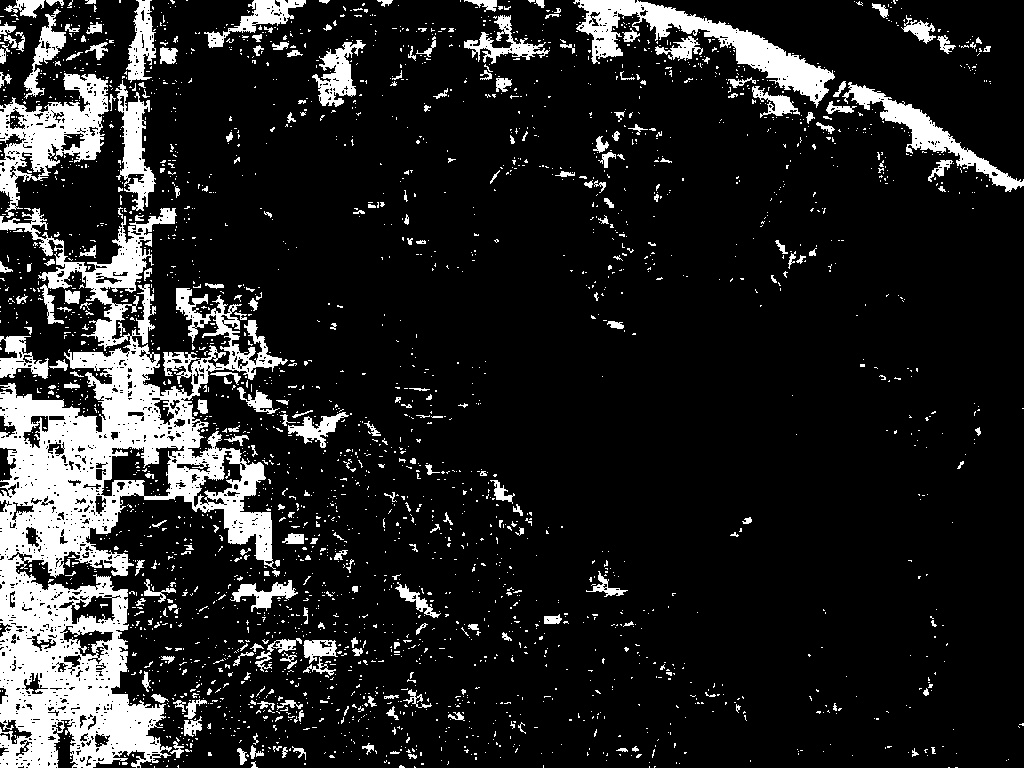
\includegraphics[scale=0.25]{Grafiken/entwicklung/4binBildHolz.jpg}
	\caption{Binärbild zeigt den Bereich des Stallbodens und Holzträgers} 
	\label{fig: Binärbild zeigt den Bereich des Stallbodens und Holzträgers}
\end{figure}

Diese zwei Binärbilder werden nun mit dem Ziel weiterverarbeitet, ein Binärbild zu erstellen, welches möglichst viele unwichtige Regionen weiss darstellt. Durch die Funktion \texttt{bitwise_or} werden die Bilder so verknüpft, dass im resultierenden Bild sämtliche Bereiche weiss sind, die in einem der beiden oder in beiden Eingangsbildern weiss sind.
\begin{figure}[H]
	\center
	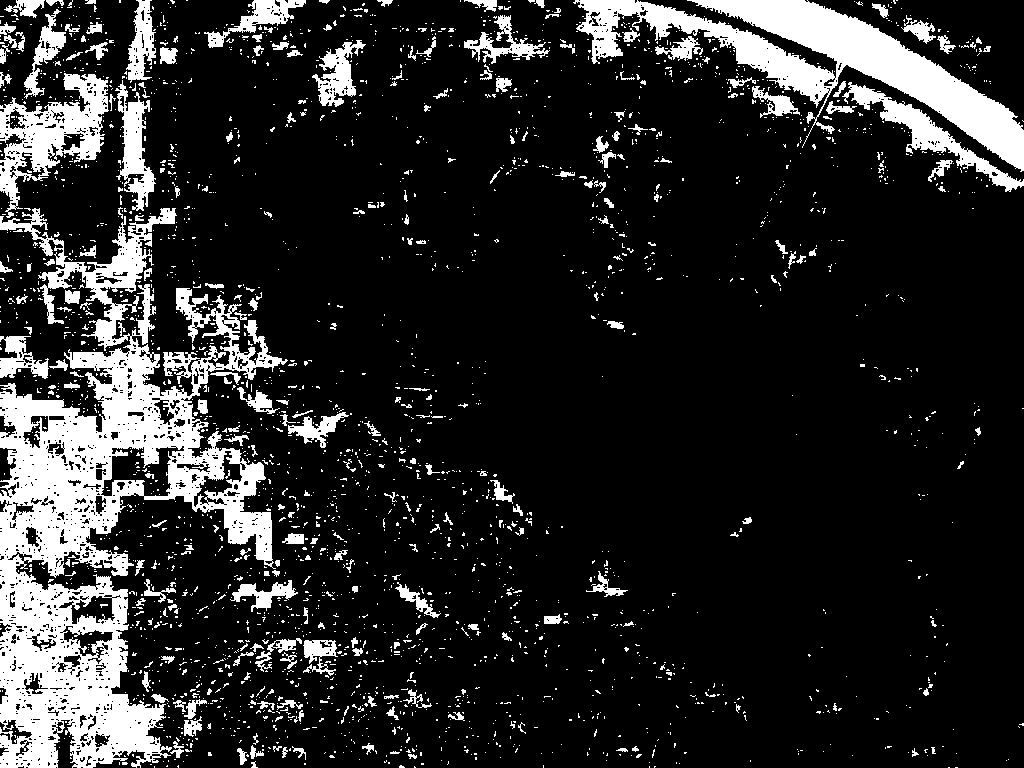
\includegraphics[scale=0.25]{Grafiken/entwicklung/5binLampeUndHolz.jpg}
	\caption{Binärbild zeigt die als unwichtig identifizierten Bereiche} 
	\label{fig: Binärbild zeigt sämtliche als unwichtig identifizierten Bereiche}
\end{figure}

Ausgehend von Abbildung \ref{fig: Binärbild zeigt sämtliche als unwichtig identifizierten Bereiche} können die als unwichtig identifizierten Bereiche als Konturen erkannt und im Originalbild eingezeichnet werden. Um dies zu erreichen, werden die Funktionen \texttt{findContours()} und \texttt{drawContours()} angewendet. Dies passiert analog zum Vorgehen bei der Detektierung von unwichtigen Bereichen. Das Resultat ist in Abbildung \ref{fig: Unwichtige Bereiche als Konturen} veranschaulicht. 
\begin{figure}[H]
	\center
	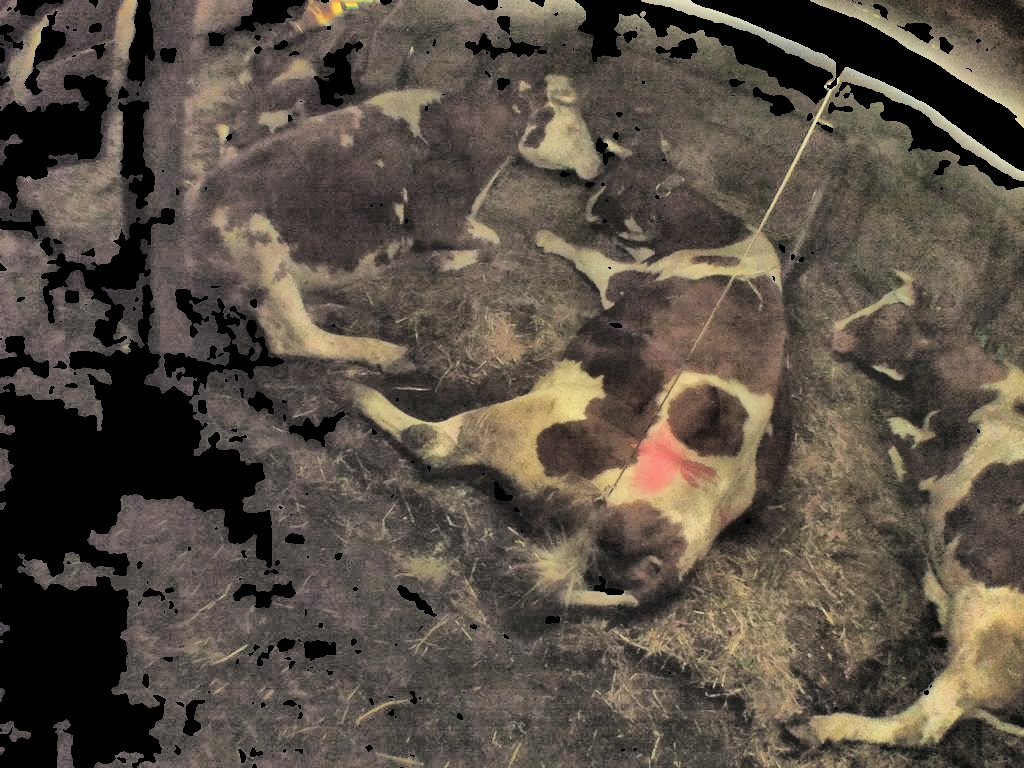
\includegraphics[scale=0.43]{Grafiken/entwicklung/6unwichtigeBereicheEingezeichnet.jpg}
	\caption{Unwichtige Bereiche  als Konturen} 
	\label{fig: Unwichtige Bereiche als Konturen}
\end{figure}

Nun gilt es, auf Basis der als unwichtig identifizierten Konturen möglichst grosse Flächen aus dem Ausgangsbild zu entfernen, respektive möglichst grosse Flächen mit schwarzer Farbe zu füllen. Um dies zu erreichen, werden mehrere Verfahren getestet. Die Abbildungen  \ref{fig: Unwichtige Bereiche als Polygone} bis \ref{fig: Unwichtige Bereiche als Rechtecke} veranschaulichen die entsprechenden Resultate unter Verwendung von OpenCV. In Abbildung \ref{fig: Unwichtige Bereiche als Polygone} wurde \texttt{approxPolyDP()} verwendet, um basierend auf den Konturen ein Vieleck zu approximieren. Die Funktion arbeitet nach dem Douglas-Peucker-Algorithmus, welcher aus einer gegebenen Kontur eine dezimierte Kontur mit weniger Punkten erstellt. Dabei kann der Funktion die maximale Distanz der originalen Kontur und ihrer Approximation als Argument mitgegeben werden \citep[S. 383]{FernandezVillan2019}.  Das Bild \ref{fig: Unwichtige Bereiche als konvexe Hülle} zeigt konvexe Hüllen der Konturen,  die als Ergebnisse der Funktion \texttt{convexHull()} entstehen. Um Kreise zu finden, welche Konturen mit möglichst geringer Fläche umschliessen, wird die Funktion \texttt{minEnclosingCircle()} verwendet (Abbildung \ref{fig: Unwichtige Bereiche als Kreise}). Zuletzt wurden für die Abbildung \ref{fig: Unwichtige Bereiche als Rechtecke} mit der Funktion \texttt{boundingRect()} Rechtecke gebildet, welche die Konturen umschliessen .

Als Vorbereitung für die Durchführung von diesen Verfahren werden Konturen mit einer Fläche von weniger als 200 Pixel gefiltert und verworfen. Die Fläche von Konturen wird mittels \texttt{contourArea()} berechnet. Durch diese erste Filterung wird erreicht, dass beispielsweise Schatten unterhalb des Schwanzes oder unterhalb der Beine der Kuh erkannt werden.
\begin{figure}[H]
	\center
	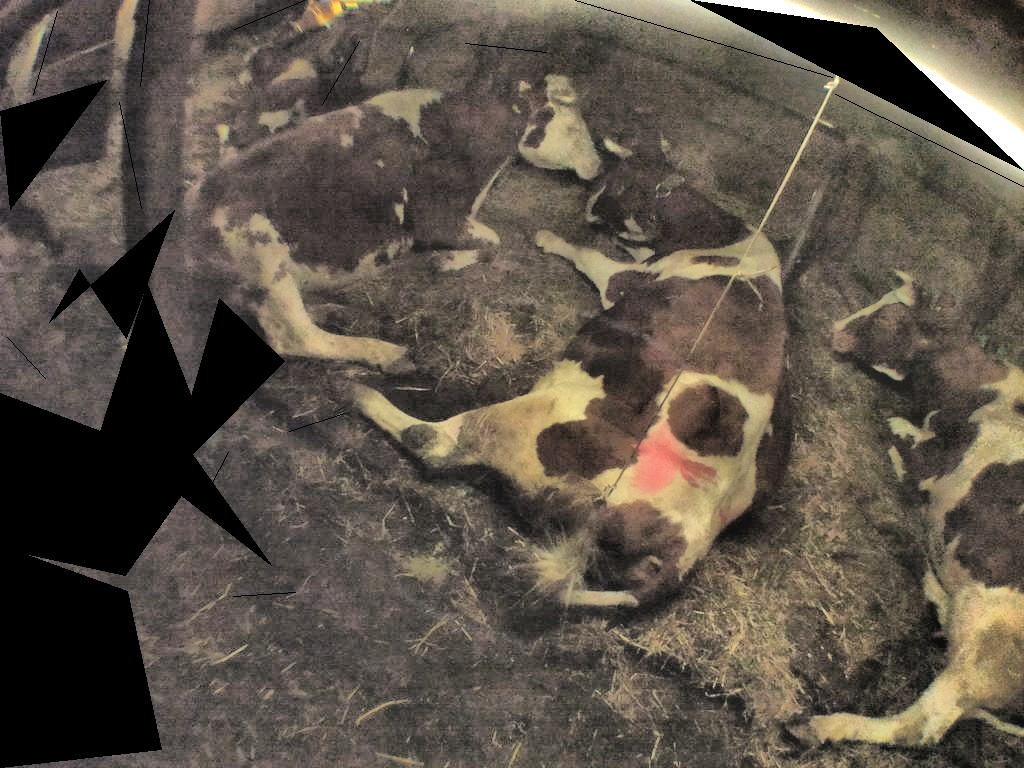
\includegraphics[scale=0.43]{Grafiken/entwicklung/7unwichtigePolygone.jpg}
	\caption{Unwichtige Bereiche als Polygone } 
	\label{fig: Unwichtige Bereiche als Polygone}
\end{figure}


\begin{figure}[H]
	\center
	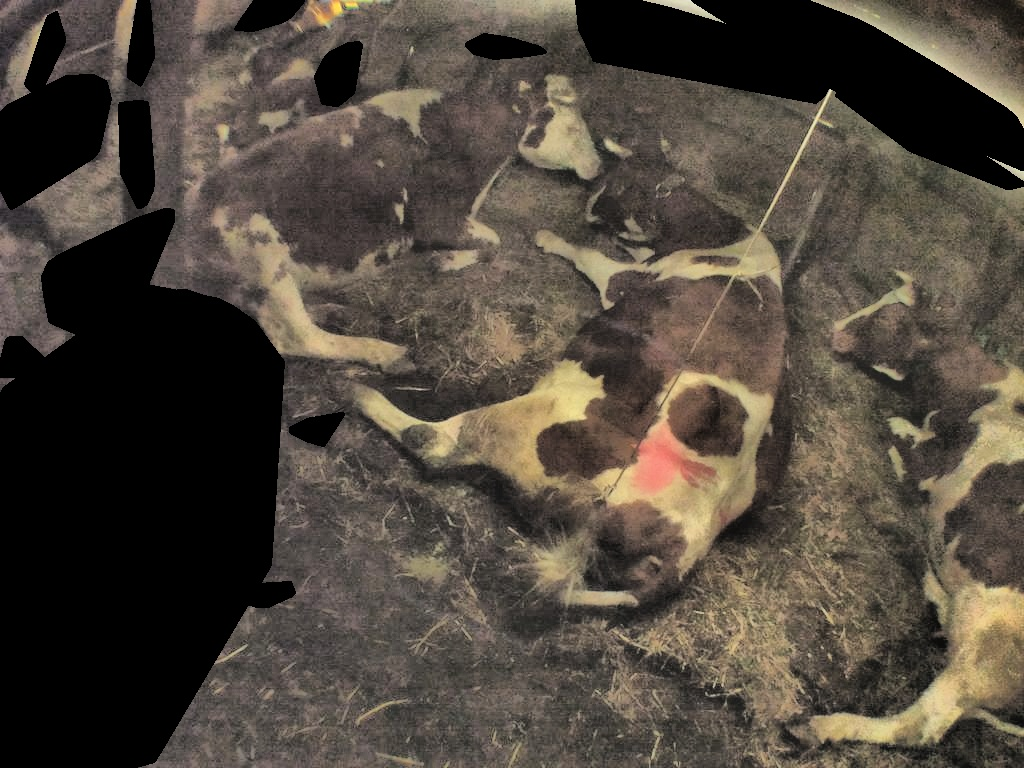
\includegraphics[scale=0.43]{Grafiken/entwicklung/7unwichtigeKonvexe.jpg}
	\caption{Unwichtige Bereiche als konvexe Hülle} 
	\label{fig: Unwichtige Bereiche als konvexe Hülle}
\end{figure}


\begin{figure}[H]
	\center
	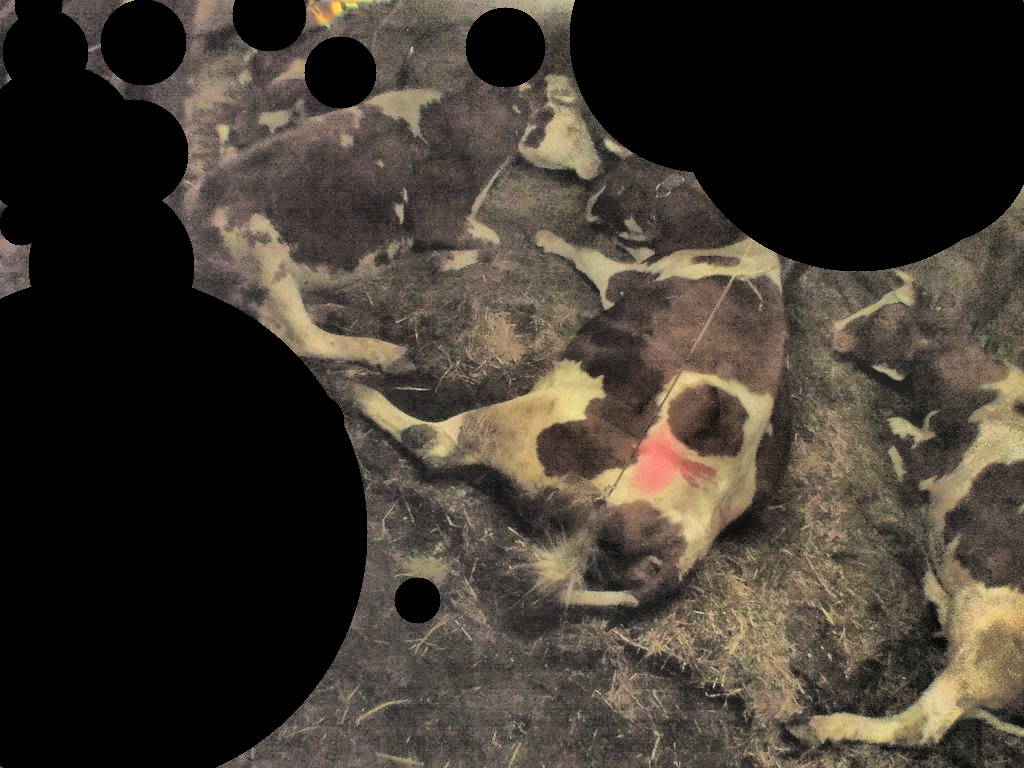
\includegraphics[scale=0.43]{Grafiken/entwicklung/7unwichtigeKreise.jpg}
	\caption{Unwichtige Bereiche als Kreise } 
	\label{fig: Unwichtige Bereiche als Kreise}
\end{figure}

\begin{figure}[H]
	\center
	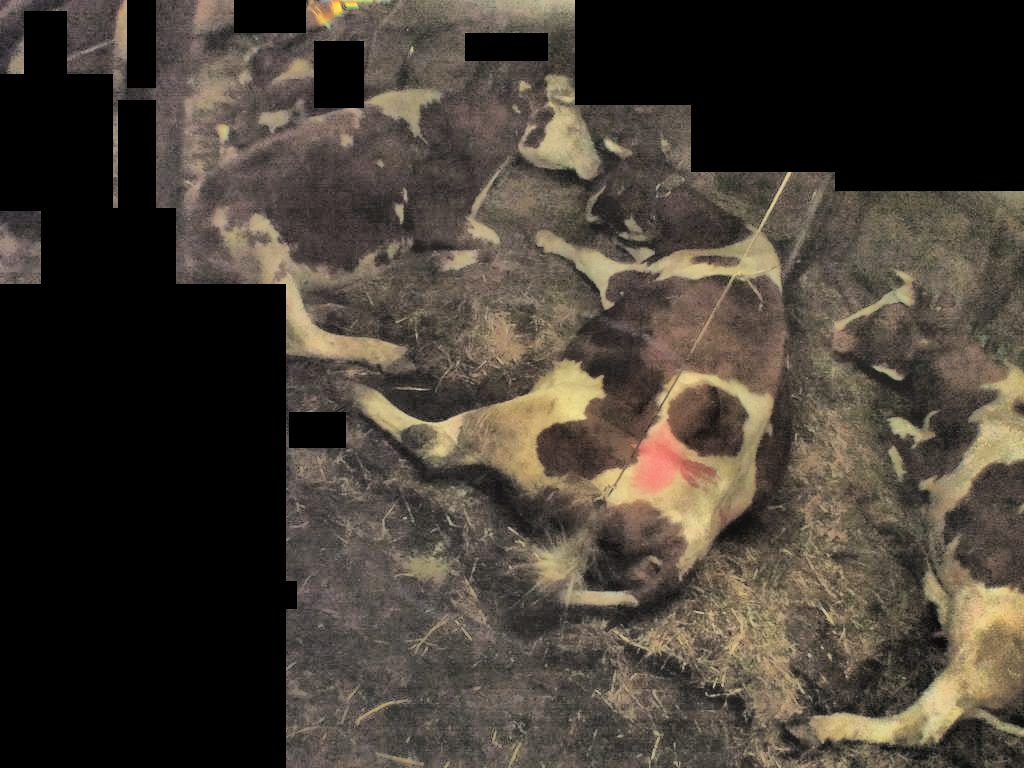
\includegraphics[scale=0.43]{Grafiken/entwicklung/7unwichtigeRechtecke.jpg}
	\caption{Unwichtige Bereiche als Rechtecke} 
	\label{fig: Unwichtige Bereiche als Rechtecke}
\end{figure}

Die Verfahren, welche mittels \texttt{minEnclosingCircle()} und \texttt{boundingRect()} angewendet werden, ergeben im vorliegenden Kontext die besten Ergebnisse. Einerseits werden die als unwichtig identifizierte Fläche wird maximiert. Andererseits werden nur sehr kleine Bereiche der Kuh fälschlicherweise als unwichtig eingestuft. Da perfekte Kreise in den Konturen von Kühen und Kälbern nicht vorkommen, entscheidet sich der Autor dafür, unwichtige Bereiche als schwarze Kreise einzuzeichnen. Zudem können diese Kreise in der weiteren Bildbearbeitung problemlos als solche erkannt werden.

\subsection{Detektierung von wichtigen Bereichen im Bild}



In einem ersten Schritt wird die geglättete und aufgehellte Version dieses Bilds mit dem adaptiven Schwellwertverfahren bearbeitet. Um dies zu erreichen, wird die Funktion \texttt{adaptiveThreshold()} mit den Argumenten \texttt{THRESH_BINARY_INV} und \texttt{ADAPTIVE_THRESH_MEAN_C} aufgerufen. Das Ergebnis dieses Versuchs, wichtige Bereiche des Bilds zu detektieren, ist in Abbildung \ref{fig: Versuch, aus geglättetem und aufgehelltem Bild wichtige Bereiche zu detektieren} ersichtlich. 

\begin{figure}[H]
	\center
	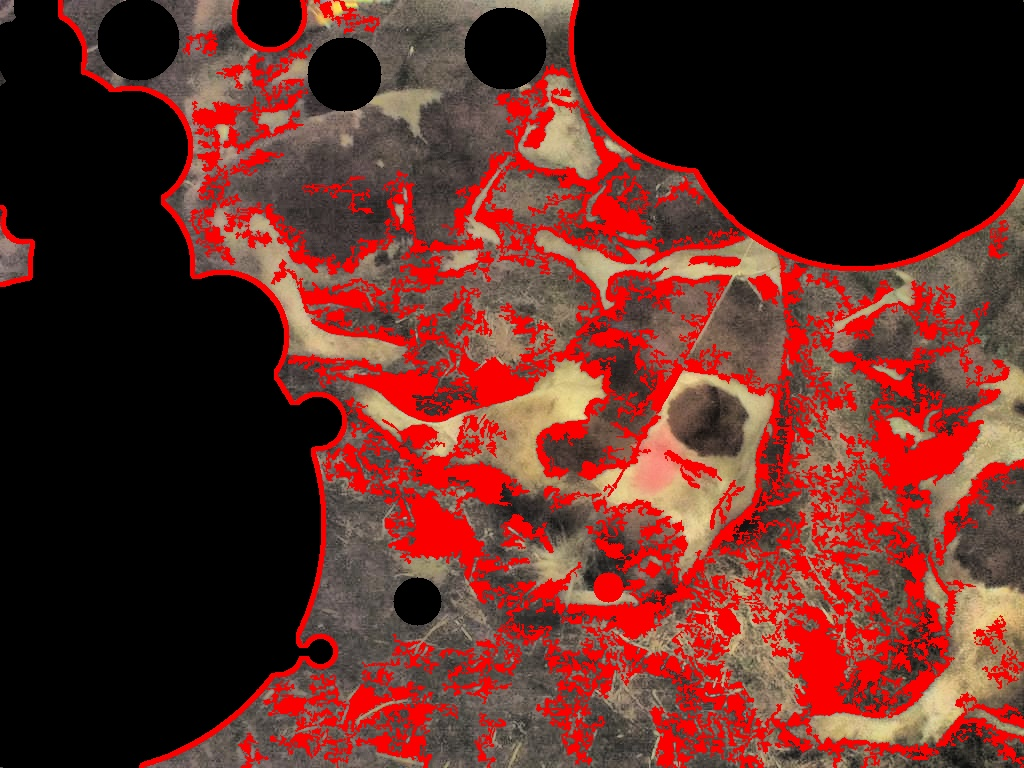
\includegraphics[scale=0.43]{Grafiken/entwicklung/10thresholdedEqualizedBirghtened.jpg}
	\caption{Versuch, aus geglättetem und aufgehelltem Bild wichtige Bereiche zu detektieren} 
	\label{fig: Versuch, aus geglättetem und aufgehelltem Bild wichtige Bereiche zu detektieren} 
\end{figure}

Das Ergebnis ist nicht brauchbar, weshalb der Versuch mit denselben Einstellungen aber mit einem nicht geglätteten Bild wiederholt wurde. Das Ergebnis ist in Abbildung \ref{fig: Versuch, aus nicht geglättetem Bild wichtige Bereiche zu detektieren} dargestellt und stellt ein besseres Zwischenergebnis dar. Als entsprechende Erkenntnis leitet der Autor ab, dass die Glättung von Histogrammen zwar die Bildqualität und Interpretationsfähigkeit für den Menschen steigert, aber im vorliegenden Kontext auch negativen Einfluss auf das Schwellwertverfahren haben kann.

\begin{figure}[H]
	\center
	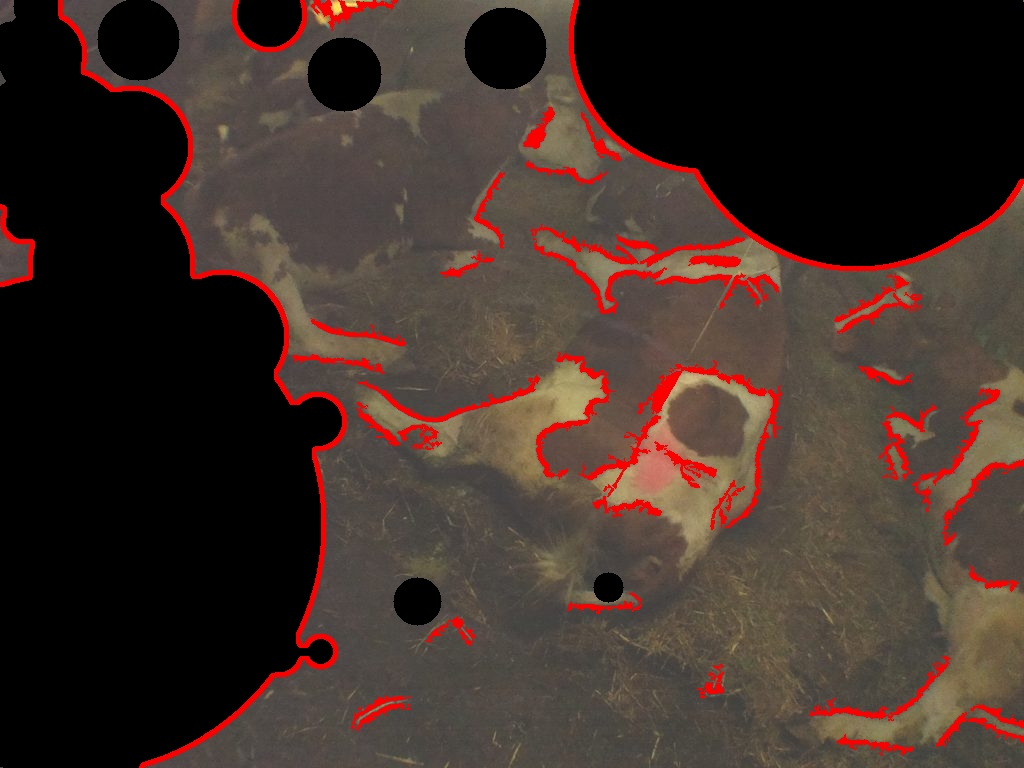
\includegraphics[scale=0.43]{Grafiken/entwicklung/11thresholdedNotEqualized.jpg}
	\caption{Versuch, aus nicht geglättetem Bild wichtige Bereiche zu detektieren} 
	\label{fig: Versuch, aus nicht geglättetem Bild wichtige Bereiche zu detektieren} 
\end{figure}

Abbildung \ref{{fig: Versuch, aus nicht geglättetem Bild wichtige Bereiche zu detektieren}} zeigt das Resultat einer vielversprechenden Analyse. Das Ergebnis ist aber insofern kritisch zu beurteilen, da die rote Farbe die gesamte Kontur ausfüllt, die detektiert wurde. Dementsprechend werden die Beine beispielsweise nicht als Kontur erkannt, sondern lediglich die Umrisse davon.
Dies dient als Motivation, die Konfiguration des Schwellwertverfahren anzupassen. Demzufolge wurde mit der Funktion \texttt{threshold()} und den Argumenten \texttt{THRESH_BINARY} als Verfahrenstyp, und dem Wert \texttt{90} als Schwellwert. Das Ergebnis daraus ist in Abbildung \ref{{fig: Ergebnisse nach angepasster Konfiguration des Schwellwertverfahrens}} dargestellt. Zudem verbessert die Filterung von kleinen Konturen die Ergebnisse weiter. Dadurch werden die als unwichtig Identifizierten Kreise und Rausch wie beispielsweise Strohhaufen neben der Kuh nicht mehr berücksichtigt.
\begin{figure}[H]
	\center
	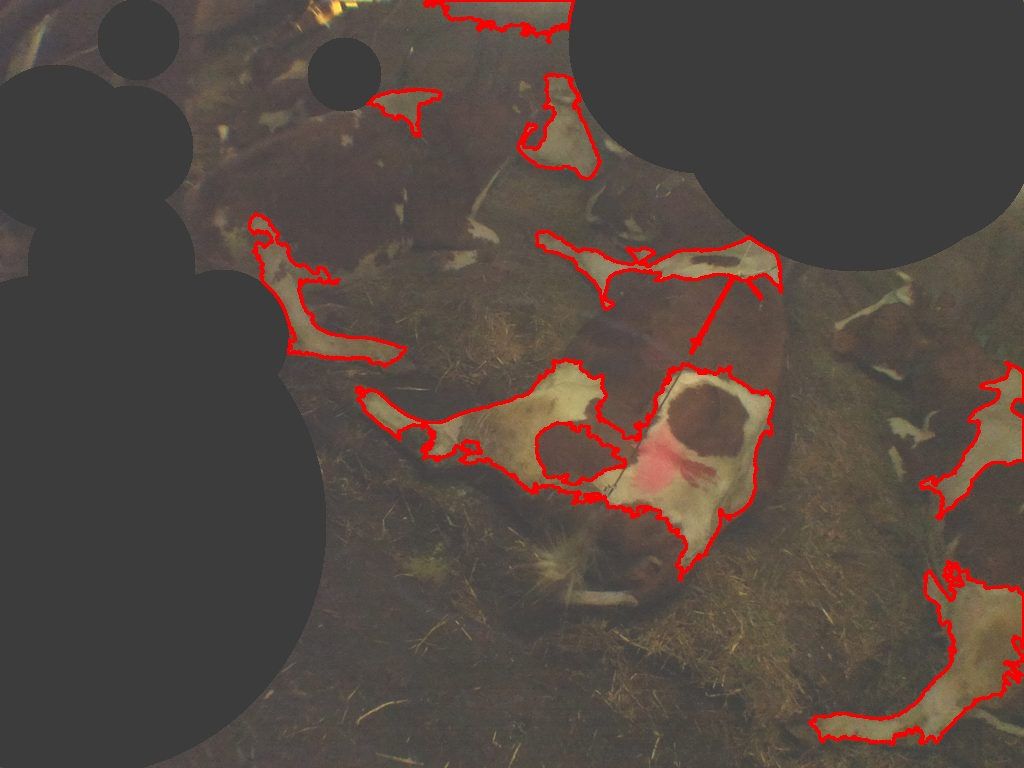
\includegraphics[scale=0.43]{Grafiken/entwicklung/12SimpleThresholdingConoturOutlineCCOMP.jpg}
	\caption{Ergebnisse nach angepasster Konfiguration des Schwellwertverfahrens} 
	\label{fig: Ergebnisse nach angepasster Konfiguration des Schwellwertverfahrens} 
\end{figure}
Es fällt nun auf, dass Flecken innerhalb der Kontur der Kuh erkannt werden. Da \texttt{findContours()} mit dem Argument \texttt{RETR_CCOMP} aufgerufen wird, werden auch Konturen innerhalb von den äusseren Konturen zurückgegeben und in eine  Hierarchie eingeteilt. Die äusseren Konturen entsprechen in den meisten Fällen den Umrissen der Kuh. Zum aktuellen Zeitpunkt reicht es aus, nur diese Umrisse zu erkennen und dementsprechend wird \texttt{findContours()} mit dem Argument \texttt{RETR_EXTERNAL} aufgerufen. Das Ergebnis ist in Abbildung  \ref{{fig: Ergebnisse nach angepasster Konfiguration des des Contour Finders}} sichtbar.
\begin{figure}[H]
	\center
	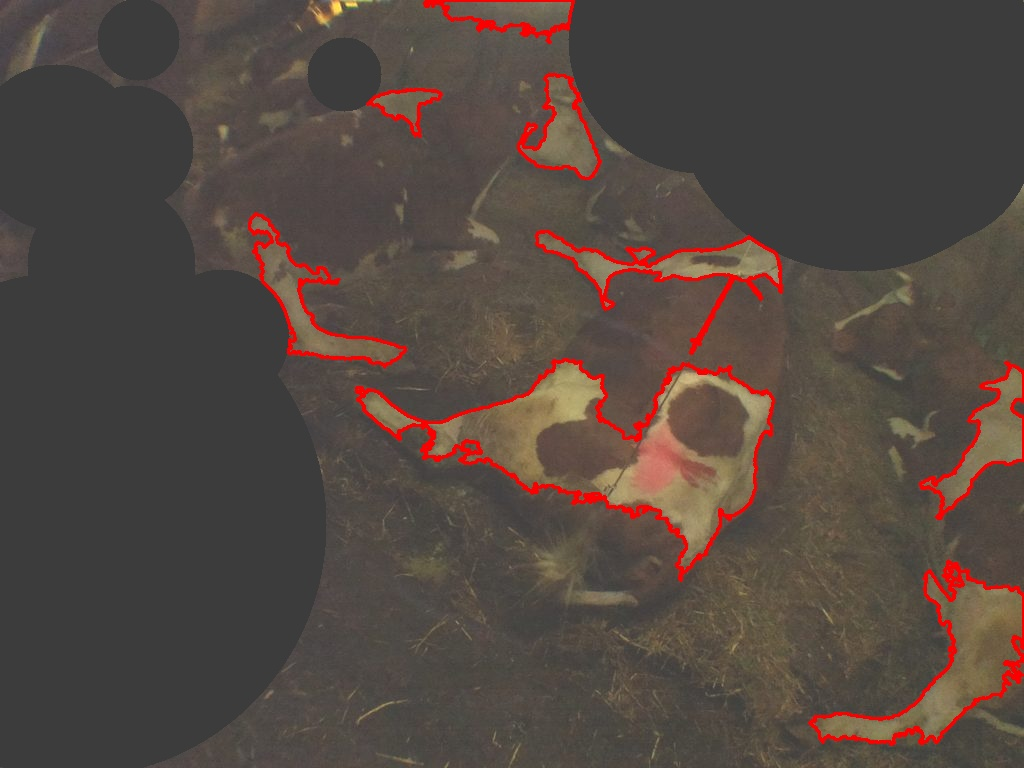
\includegraphics[scale=0.43]{Grafiken/entwicklung/13SimpleThresholdingConoturOutlineLIST.jpg}
	\caption{Ergebnisse nach angepasster Konfiguration des des Contour Finders} 
	\label{fig: Ergebnisse nach angepasster Konfiguration des des Contour Finders} 
\end{figure}

Dabei unterscheiden sich die Ergebnisse bei der Anwendung von \texttt{findContours()} mit unterschiedlichen Approximationsverfahren wie \texttt{CHAIN_APPROX_SIMPLE}, \texttt{CHAIN_APPROX_TC89_L1}, \texttt{CHAIN_APPROX_TC89_KCOS} von der Deaktivierung der Approximation  nicht wesentlich. Auch unterschiedliche Modi wie \texttt{RETR_LIST} oder \texttt{RETR_CCOMP} für die Identifizierung der Konturen ergeben in diesem Kontext identische Ergebnisse. Es werden jeweils die neun eingezeichneten Konturen identifiziert.



\begin{figure}[H]
	\center
	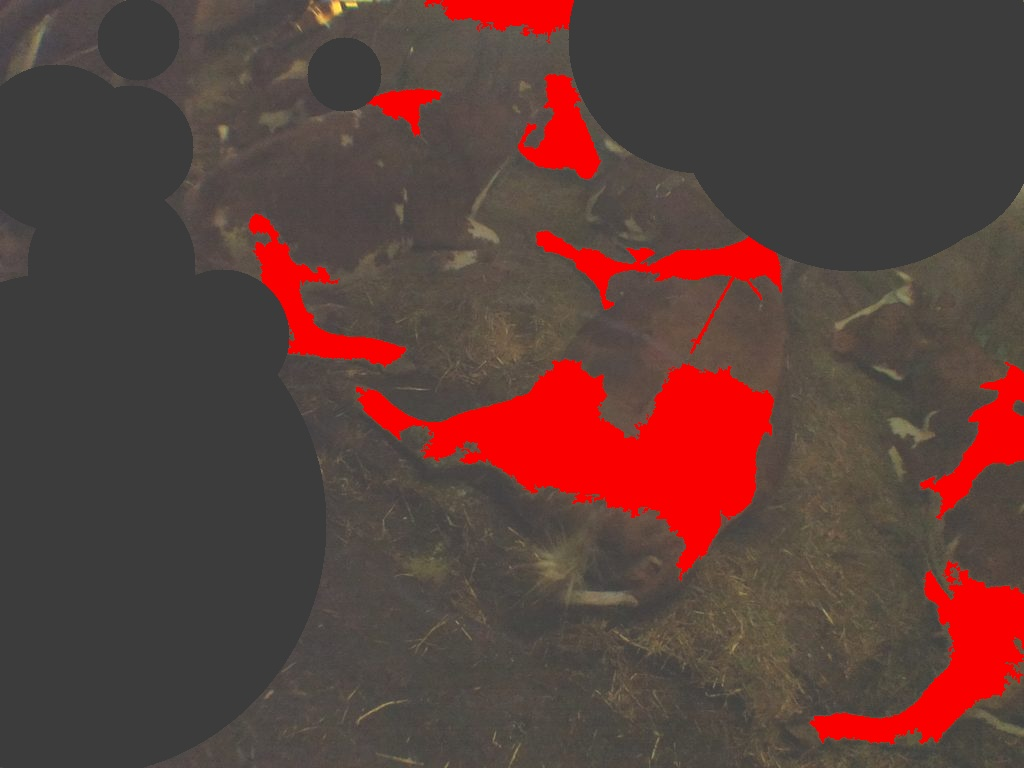
\includegraphics[scale=0.43]{Grafiken/entwicklung/14AfterThresholdingContourFilled.jpg}
	\caption{Konturen mit Farbe gefüllt} 
	\label{fig: Konturen mit Farbe gefüllt} 
\end{figure}


\subsection{Erkennung von seitlich liegender Kuh}
Aus der Domänenanalyse und Experteninterviews hat sicher ergeben, dass seitliches Liegen ein starkes Geburtsanzeichen ist und entsprechend detektiert werden muss. Die Seitenlage charakterisiert sich unter anderem mit gestreckten Beinen. Um diese zu erkennen, 
Um die detektierten Konturen weiter einzugrenzen, werden diese nach entsprechenden Winkeln gefiltert. 

Da nun lediglich äussere Konturen detektiert werden, dürfen diese Konturen mit Farbe gefüllt werden, ohne relevante Informationen über Hierarchien zu vernichten (Abbildung \ref{fig: Konturen mit Farbe gefüllt und Filterung von Konturen unterhalb Minimalgrösse}). Da nun keine weiteren Konturen mehr gesucht werden (kein Aufruf von \texttt{findContours()}), sind nachfolgend sämtliche dargestellten Bilder bearbeitet, um deren Helligkeit und Kontrast zu erhöhen. Dies wurde unter Anwendung der Funktionen \texttt{add()} und \texttt{createCLAHE()} gemacht . Zudem wurden die schwarze Kreise, welche unwichtige Bereiche des Bildes verdecken entfernt. Dies erhöht die Lesbarkeit des Berichts.

\begin{figure}[H]
	\center
	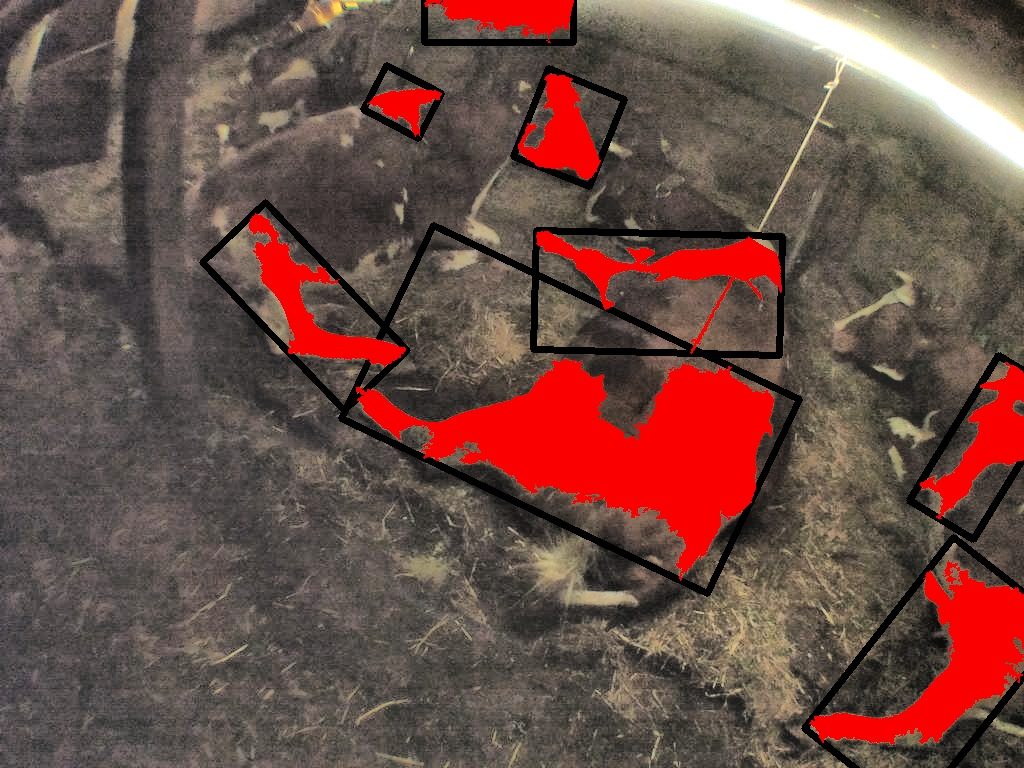
\includegraphics[scale=.43]{Grafiken/entwicklung/20StartImage.jpg}
	\caption{Ausgangslage vor der Analyse und Filterung der Konturen} 
	\label{fig: Ausgangslage vor der Analyse und Filterung der Konturen} 
\end{figure}

\subsubsection{Erkennung der Beine anhand von Winkel}
\begin{figure}[H]
	\center
	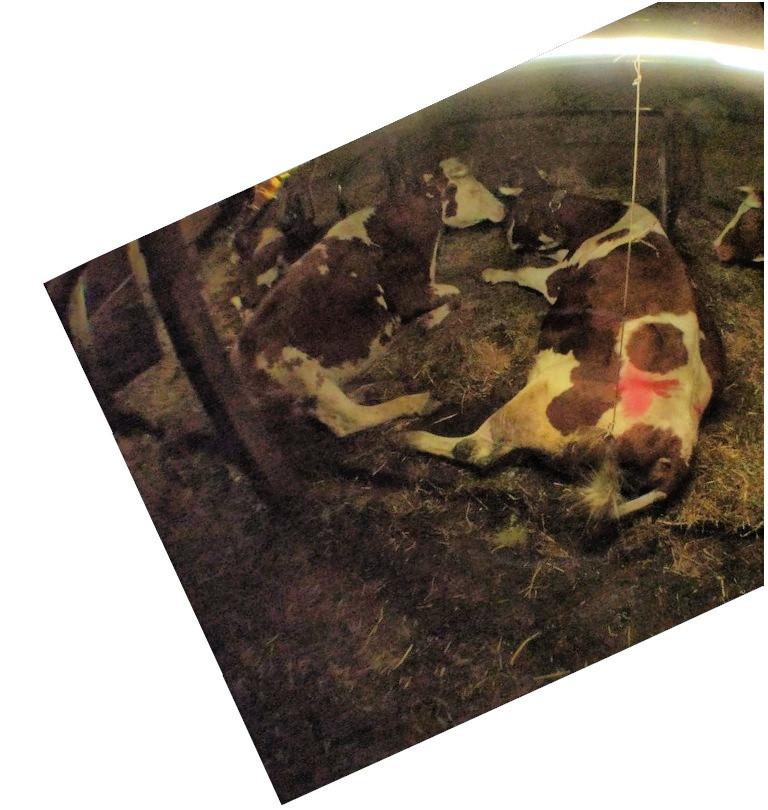
\includegraphics[scale=1.3]{Grafiken/entwicklung/21AngleCorrecturDemonstration.jpg}
	\caption{Veranschaulichung zur Analyse der Winkel} 
	\label{fig: Veranschaulichung zur Analyse der Winkel} 
\end{figure}


Dabei entspricht das ungefähr einer Rotation des Bildes... blbla gemäss Notizen
noch erklären, dass ich für positiven und negativen winkel genau dasselbe wiederholt habe.

\begin{figure}[H]
	\center
	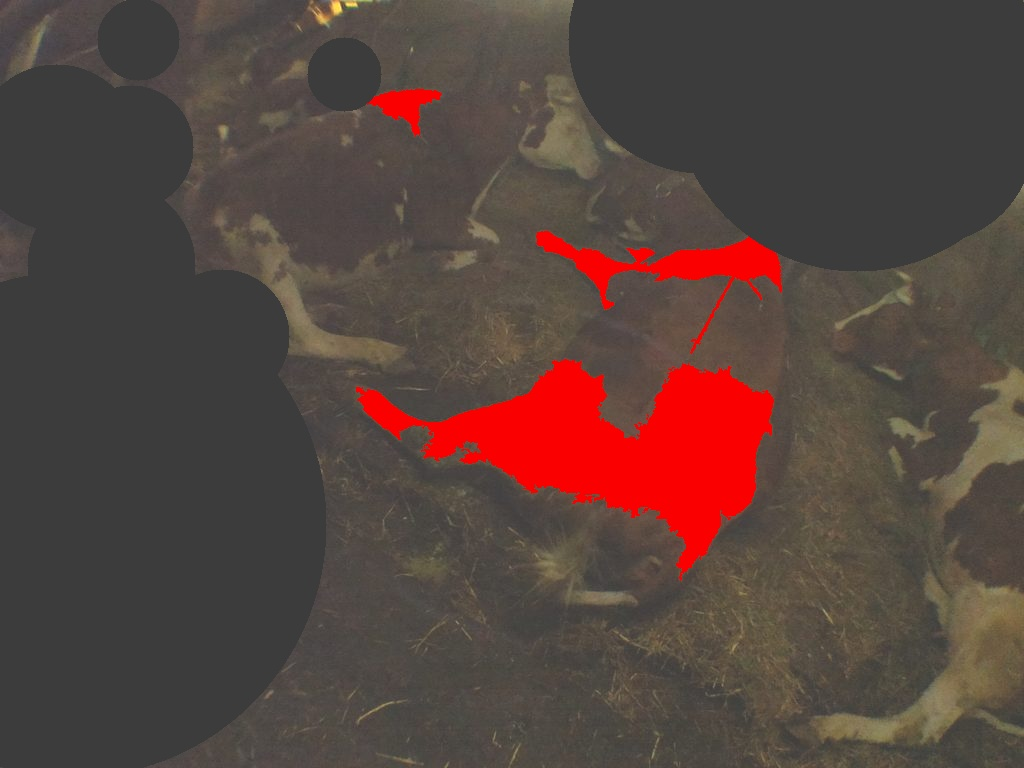
\includegraphics[scale=0.43]{Grafiken/entwicklung/22AngleCorrectur.jpg}
	\caption{Ergebnisse nach Filterung der Konturen nach Winkel} 
	\label{fig: Ergebnisse nach Filterung der Konturen nach Winkel} 
\end{figure}
\subsubsection{Erkennung der Beine anhand von Extent}
Um diese Ergebnisse weiter zu analysieren, wurde mittels \texttt{minAreaRect()} ein für jede Kontur das Rechteck ermittelt, welches mit der kleinsten Fläche sämtliche Punkte der Kontur einschliesst \ref{fig: Rechteck mit kleinsten Fläche, welches die Kontur einschliesst}.  


Bei Betrachtung dieser Rechtecke stellt der Autor die Vermutung auf, dass sich die Beine der Kuh insbesondere bei zwei Eigenschaften stark von der weiteren, unerwünschten Kontur unterscheidet. 



Zuerst wird da Verhältnis zwischen der Fläche der erkannten Kontur und der Fläche des Rechtecks, das die Kontur einschliesst betrachtet. Dieses Verhältnis wird nachfolgend Extent genannt.


Abbildung \ref{fig :Verhältnis zwischen Konturfläche und der Fläche des Rechtecks, welches die Kontur einschliesst} verdeutlicht, dieses Verhältnis zwischen der roten Flächen und der Fläche der schwarzen Rechtecke.  Der Autor erwartet, dass die Kontur der Beine gegenüber dem darum gebildeten Rechteck klein ist. Entsprechend wird für als Extent bei Beinen einen tiefen Wert angenommen im Vergleich zum Wert des Extent bei anderen Figuren. Dementsprechend wäre die Definition eines Maximalen Schwellwertes denkbar, die ermittelt, ob es sich bei einer betrachteten Kontur um die Beine handelt. 



\begin{equation}\label{Extent}
Extent =  \frac{Fl\ddot{a}che\ der\ Kontur}{Fl\ddot{a}che\  umschliessendes\  Rechteck}  
\end{equation}

Nun wird als Schwellwert für Extent \texttt{0.35} angenommen und entsprechend werden nur noch Konturen berücksichtigt, welche unterhalb dieses Werts liegen. In Abbildung \ref{fig: Ergebnis der Filterung der Konturen nach Winkel und Extent}sind alle Konturen mit ${Extent < 0.35}$ rot und alle Konturen mit $Extent \geq 0.35 $ grün eingefärbt. Der Autor stellt fest, dass der Wert für den Extent der unerwünschten Kontur zwischen den beiden Extenten der beiden Konturen der Beine liegt. Also ist in diesem Bild eine Klassifikation von Beinen und unerwünschten Konturen nicht möglich. 




\begin{figure}[H]
	\center
	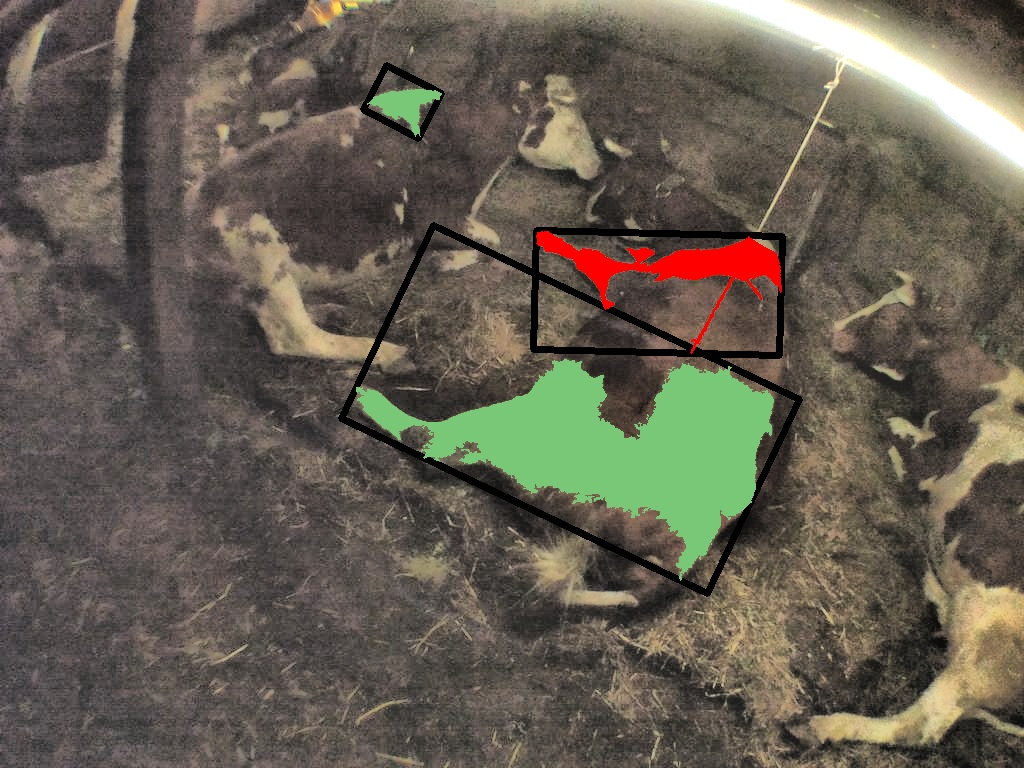
\includegraphics[scale=0.43]{Grafiken/entwicklung/25ExtentDemonstration.jpg}
	\caption{Ergebnis der Filterung der Konturen nach Winkel und Extent } 
	\label{fig: Ergebnis der Filterung der Konturen nach Winkel und Extent} 
\end{figure}

Um die Klassifikation mittels Extent weiter zu verfolgen, wird mit dem Schwellwert \texttt{35} eine Klassifikation sämtlicher Konturen vorgenommen. Also auch der Konturen, welche bereits aufgrund des Winkels klassifiziert wurden. Das Ergebnis ist in Abbildung \ref{fig: Ergebnis der Filterung der Konturen nach Extent} sichtbar. Nach wie vor sind Konturen mit \texttt{Extent < 0.35} rot und alle Konturen mit \texttt{Extent >= 0.35} grün eingefärbt. Abbildung \ref{fig: Ergebnis der Filterung der Konturen nach Extent} veranschaulicht, dass dennoch sechs von acht Konturen korrekt klassifiziert wurden. Auf Basis dessen entscheided sich der Autor, eine Filterung der Konturen umzusetzen mit dem Schwellwert  \texttt{40}. Dies erlaubt, Konturen wie den Kopf der Kuh auszuschliessen und macht dementsprechend das Ergebnis stabiler.
\begin{figure}[H]
	\center
	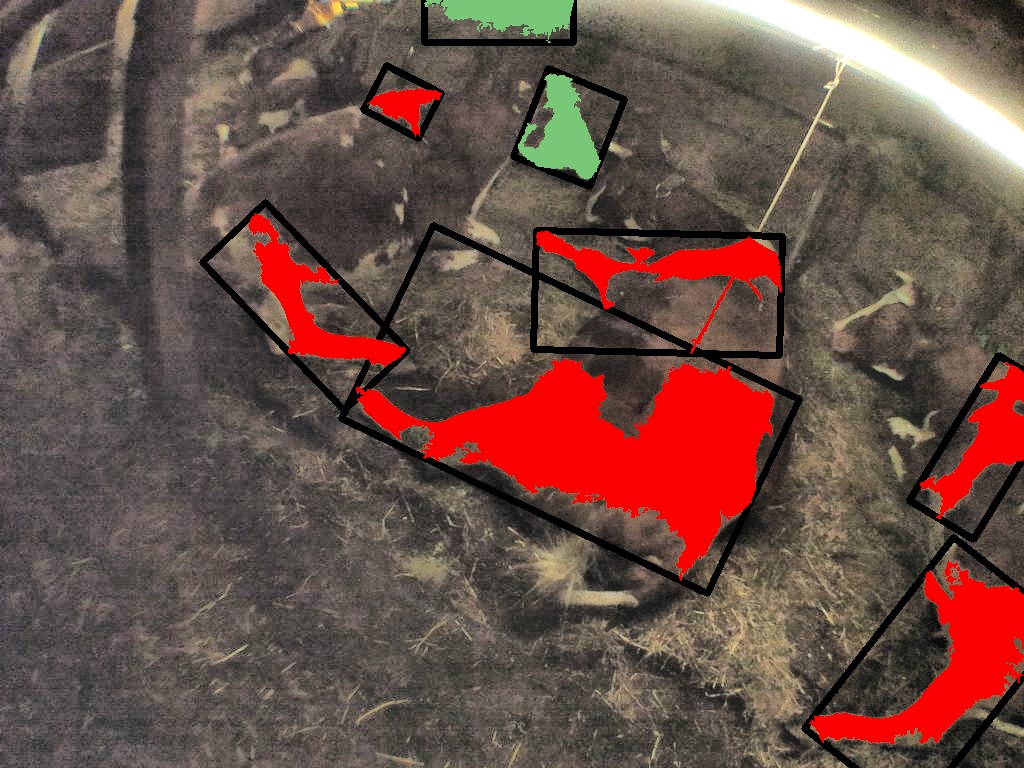
\includegraphics[scale=0.43]{Grafiken/entwicklung/26FilteringExtent.jpg}
	\caption{Ergebnis der Filterung der Konturen nach Extent:SCHWELLWERT = 0.5 } 
	\label{fig: Ergebnis der Filterung der Konturen nach Extent} 
\end{figure}
\subsubsection{Erkennung der Beine anhand von Aspect Ratio}

Rechtecke, welche die Beine der Kuh einschliessen sind langgezogen. Der Autor überprüft nun die Vermutung, dass diese Eigenschaft dabei hilf, Beine von unwichtigen Konturen zu unterscheiden. Das Verhältnis zwischen Breite und Höhe der Rechtecke (nachfolgend Aspect Ratio genannt) liefert Informationen darüber, wie langgezogen ein Rechteck ist.	
	
\begin{equation}\label{Extent}
Aspect Ratio =  \frac{Breite}{H\ddot{}he}  
\end{equation}
Damit der Vergleich der Aspect Ratio einfacher ist wird die Formel etwas angepasst.
\begin{equation}\label{Extent}
Aspect Ratio =  \frac{Lange \ Seite}{kurze \ Seite}  
\end{equation}
Durch Filterung der Konturen mit dem Schwellwert \texttt{1.5} können Konturen demnach gefiltert werden, wenn deren umschliessendes Rechteck einem Quadrat ähnlich sieht. Das Ergebnis dieser Filterung ist in Abbildung \ref{{fig: Ergebnis der Filterung der Konturen nach Aspect Ratio}} sichtbar.
\begin{figure}[H]
	\center
	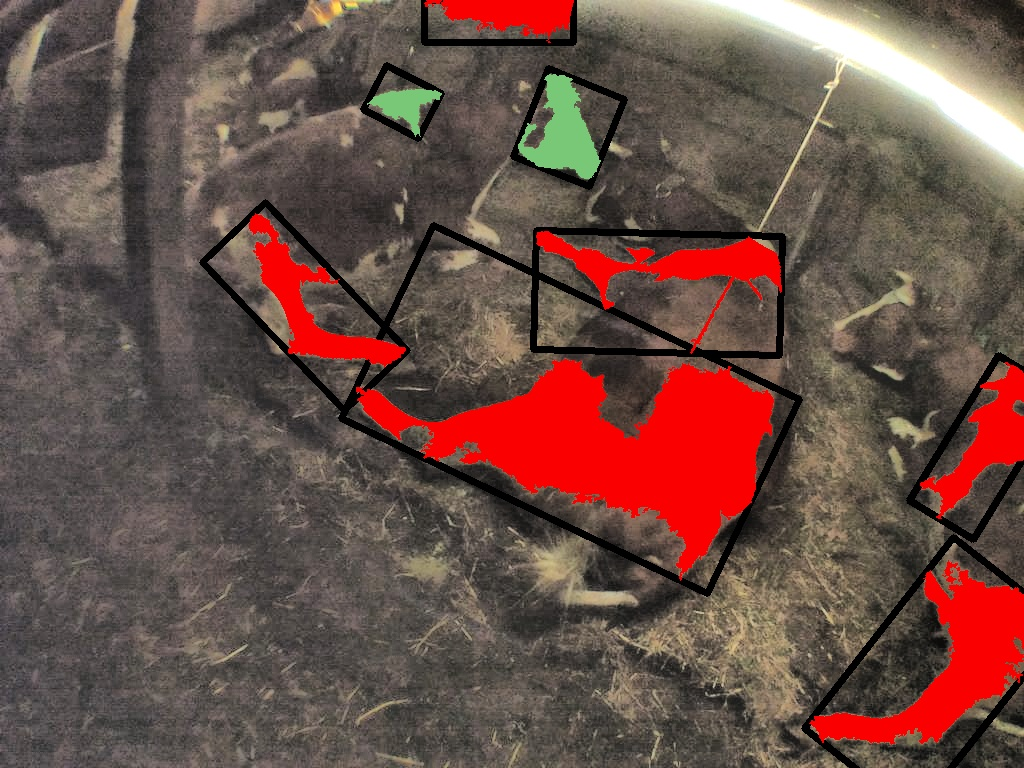
\includegraphics[scale=0.43]{Grafiken/entwicklung/27AspectRatio.jpg}
	\caption{Ergebnis der Filterung der Konturen nach Aspect Ratio } 
	\label{fig: Ergebnis der Filterung der Konturen nach Aspect Ratio Schwellwert=1.5} 
\end{figure}

Wenn man die Resultate der Filterung durch Winkel, Extent und Aspect Ratio kombiniert, erreicht man das Resultat gemäss Abbildung \ref{fig: Ergebnis der Filterung der Konturen nach Winkel, Extent und Aspect Ratio}. Dabei werden Winkel zwischen 80 und 110 Grad, Extent unter 0.4 und Aspect Ratios über 1.5 berücksichtigt.



\begin{figure}[H]
	\center
	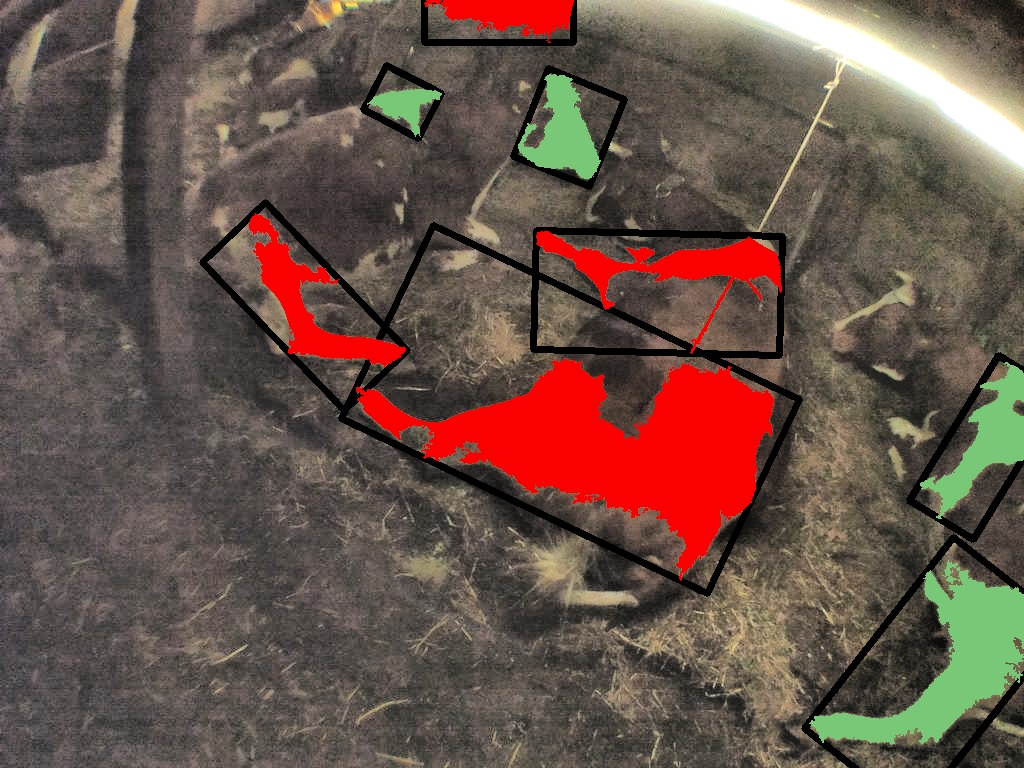
\includegraphics[scale=0.43]{Grafiken/entwicklung/28FilteredAspectAndAngle.jpg}
	\caption{Ergebnis der Filterung der Konturen nach Winkel und Aspect Ratio} 
	\label{fig: Ergebnis der Filterung der Konturen nach Winkel, Extent und Aspect Ratio} 
\end{figure}

Nun werden vier Konturen als potentielle Konuturen von Beinen bei seitlichem Liegen erkannt. Wünschenswert wäre nun, diese Auswahl weiter einzugrenen. Nun ist es wünschenswert, eine Gemeinsamkeit Konturen der Beine der mittleren Kuh zu erkennen. Um die beiden Figuren zu vergleichen, wurde die Funktion \texttt{matchShapes()} eingesetzt. Dabei wurde jede Kontur mit jeder anderen Kontur verglichen und zwei sehr ähnliche Figuren wurden ausgewählt. Leider hat der Algorithmus nicht das gewünschte Resultat bewirkt (Abbildung \ref{fig: Ergebnis der Shape Matching}). 

\begin{figure}[H]
	\center
	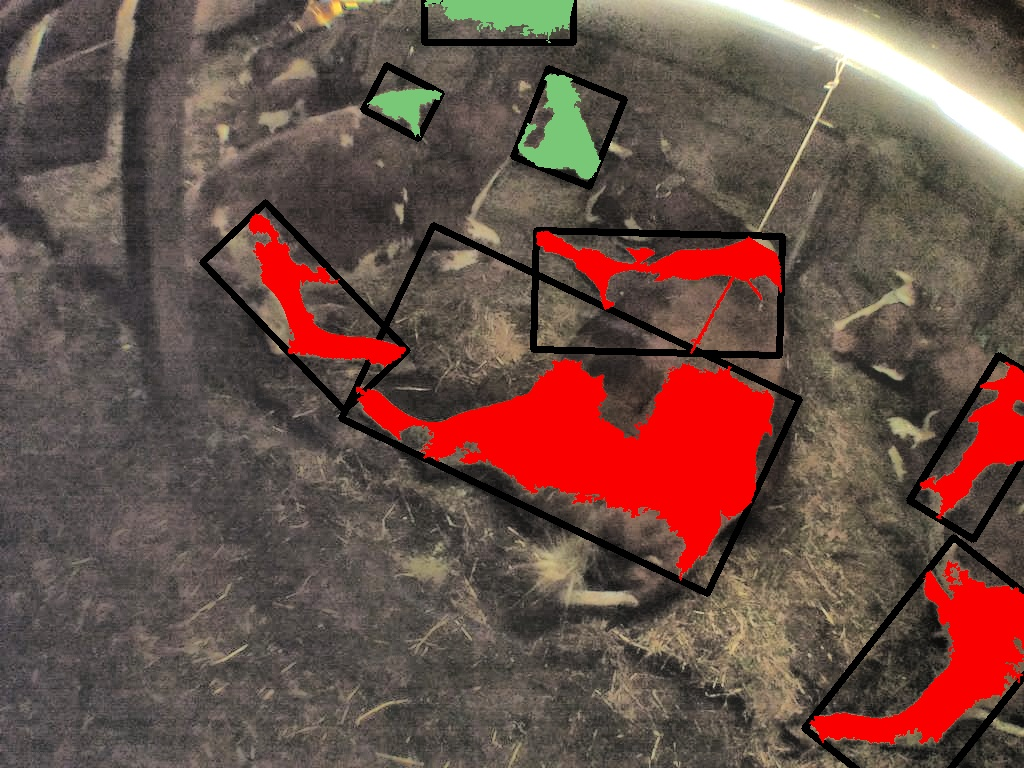
\includegraphics[scale=0.43]{Grafiken/entwicklung/29FilteredByExtentAndAspect.jpg}
	\caption{Ergebnis der Filterung der Konturen nach Extent und Aspect Ratio} 
	\label{fig: Ergebnis der Filterung der Konturen nach Extent und Aspect Ratio} 
\end{figure}

\begin{figure}[H]
	\center
	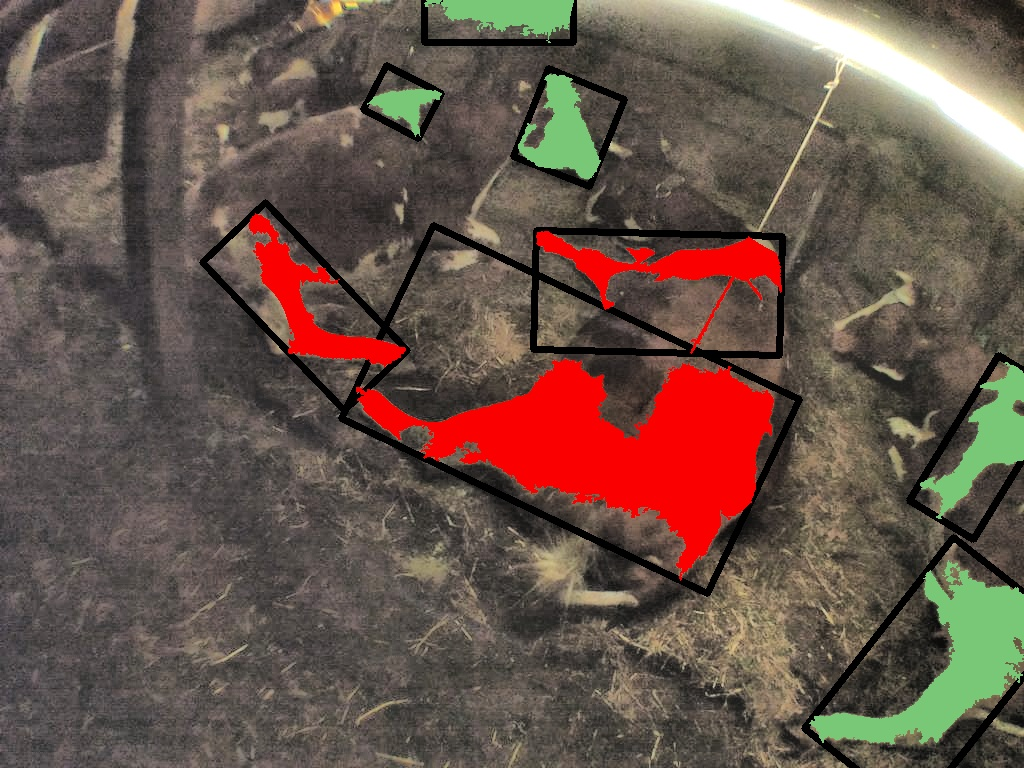
\includegraphics[scale=0.43]{Grafiken/entwicklung/30FilteredByExtentAspectAngle.jpg}
	\caption{Ergebnis der Filterung der Konturen nach Winkel, Extent und Aspect Ratio} 
	\label{fig: Ergebnis der Filterung der Konturen nach Extent und Aspect Ratio} 
\end{figure}

\begin{figure}[H]
	\center
	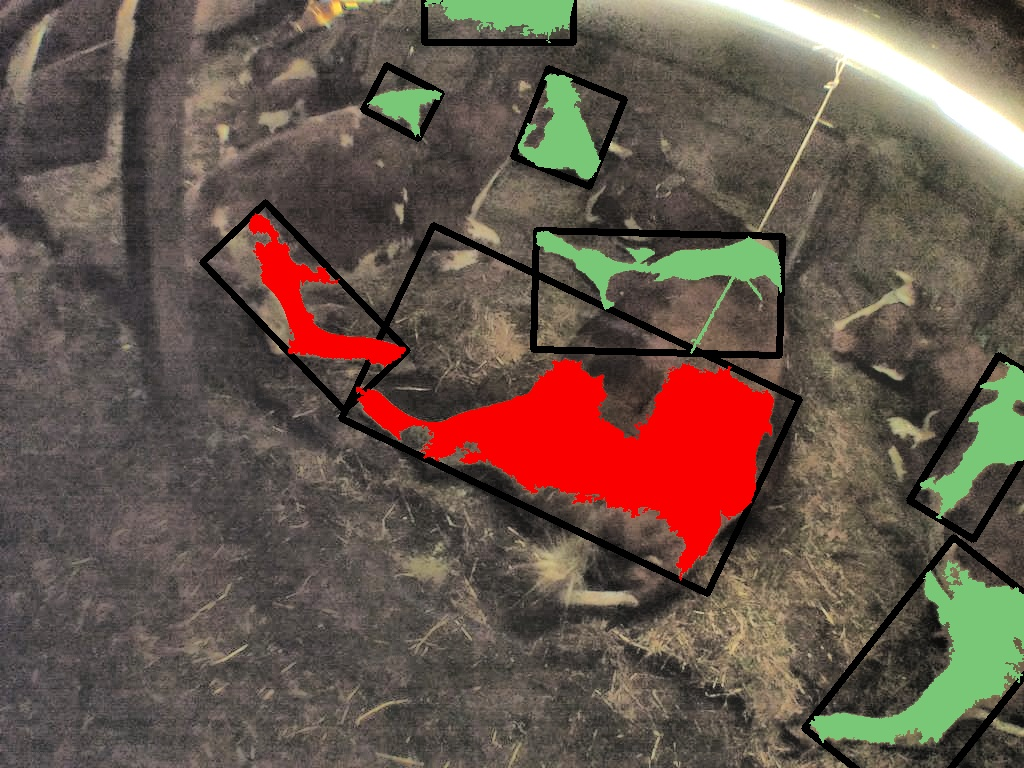
\includegraphics[scale=0.43]{Grafiken/entwicklung/31FilteredBySimilarity.jpg}
	\caption{Ergebnis der Shape Matching} 
	\label{fig: Ergebnis der Shape Matching} 
\end{figure}

Um sicherzustellen, dass dieses Resultat nicht auf die Winkel der Konturen zurückzuführen sind (die Winkel wurden ja bereits bereinigt), verschiebt der Autor sämtliche Winkel auf 60 Grad und vergleicht die Konturen wieder mit \texttt{matchShapes()} und Schwellwert 2. Das Ergebnis ist dasselbe, die Klassifikation kann zu diesem Zeitpunkt nicht mehr verbessert werden. 
\begin{figure}[H]
	\center
	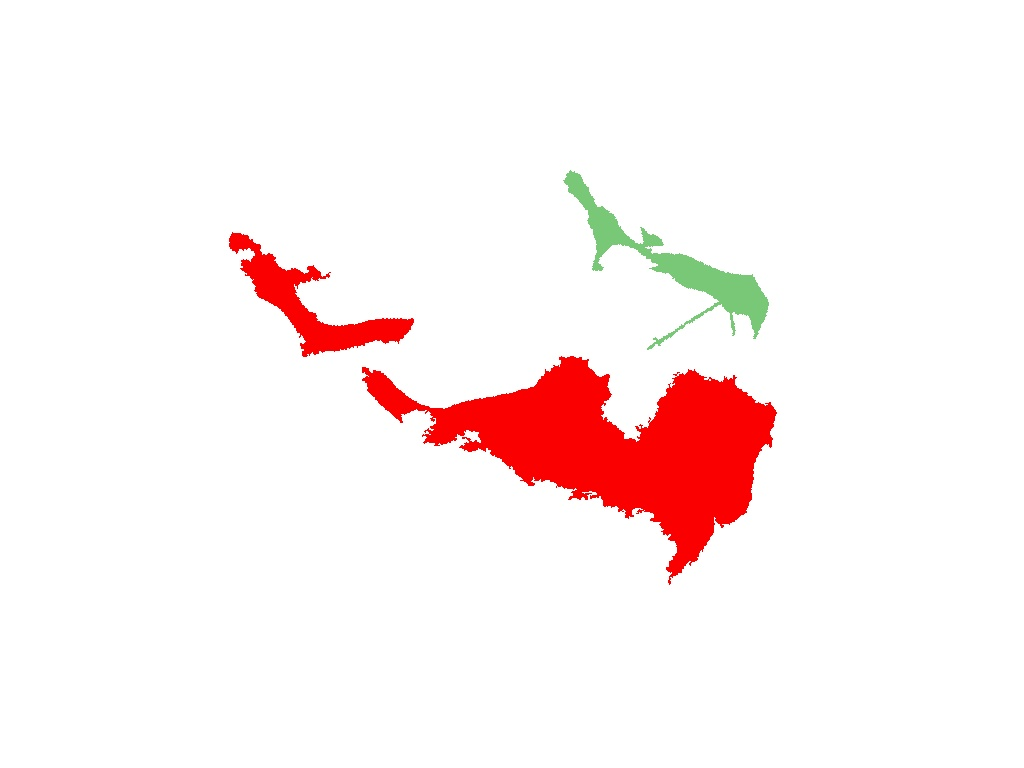
\includegraphics[scale=0.43]{Grafiken/entwicklung/32BlankFilteredBySimilarity.jpg}
	\caption{Ergebnis der Shape Matching und Korrektur der Winkel} 
	\label{fig: Ergebnis der Shape Matching und Korrektur der Winkel} 
\end{figure}


Mit einem Schwellwert von 3 kann jedoch das Resultat weiter stabilisiert werden.
